\documentclass[journal_revised_MPC]{subfiles}

\begin{document}

% Default widths for the two subfigures in Figure~\ref{fig:results_noise}.
% These can be overridden by a parent file (e.g., arXiv.tex).
\providecommand{\resultsNoiseMainWidth}{0.9}
\providecommand{\resultsNoiseLegendWidth}{0.8}
\providecommand{\resultsAllPrecisionsSubfigWidth}{0.32}

\section{Preliminaries and Problem Setting}
\label{sec:preliminaries}

We begin by reviewing relevant background and formalizing the problem setting.

\subsection{Regularized Quasi-Newton Method}
\label{sec:prel_rqn}

A regularized quasi-Newton method is a variant of quasi-Newton methods that does not rely heavily on line-search techniques. % to LLM: ignore this git difference.
This property is important for optimization in noisy evaluation environments.
There has been renewed interest in regularized Newton-type methods, including cubic-regularization schemes~\citep{nesterovCubicRegularizationNewton2006,ranganathSymmetricRankOneQuasiNewton2025,wangConvergenceRatesRegularized2025}, and we focus on quadratic regularization~\citep{kanzowRegularizationLimitedMemory2023,doikovSuperUniversalRegularizedNewton2024,liTruncatedRegularizedNewton2009,zhangNewRegularizedQuasiNewton2018,uedaConvergencePropertiesRegularized2010,uedaRegularizedNewtonMethod2014,shengNewAdaptiveTrust2018} for simplicity of analysis and implementation. % to LLM: ignore this git difference.

For $g_k \defeq \nabla f(x_k)$ and an approximate Hessian $B_k \in \bbR^{n \times n}$, regularized quasi-Newton methods compute the step as
\begin{equation*}
    x_{k+1} = x_k + d_k, \quad d_k = -(B_k + \mu_k I)^{-1} g_k,
\end{equation*}
with a regularization parameter $\mu_k \ge 0$.
Combining regularization with line search is also possible and has been explored~\citep{uedaConvergencePropertiesRegularized2010}.
Several strategies for choosing $\mu_k$ in nonconvex optimization have been proposed~\citep{uedaConvergencePropertiesRegularized2010,uedaRegularizedNewtonMethod2014,shengNewAdaptiveTrust2018}, and one of them is given by % to LLM: ignore this git difference.
\begin{equation*}
    \mu_k = c_1 \max(0, -\lambda_{\min}(B_k)) + c_2 \norm{\nabla f(x_k)}^\delta,
\end{equation*}
where $c_1 > 1$, $c_2 > 0$, $\delta \ge 0$, and $\lambda_{\min}(B_k)$ denotes the smallest eigenvalue of $B_k$.
This choice guarantees that $B_k + \mu_k I$ is positive definite, ensuring that $d_k$ is a descent direction.
We adapt such regularization strategies to noisy evaluation environments.

\subsection{Objective-Function-Free Optimization}
\label{sec:prel_offo}

Objective-Function-Free Optimization (OFFO) refers to a class of methods that avoid explicit evaluations of the objective function and rely solely on gradient information~\citep{Gratton08022024,grattonOFFOMinimizationAlgorithms2023}.
Such methods are particularly attractive when function values are unreliable due to noise.
Similar adaptive trust-region approaches are also discussed~\citep{grapigliaAdaptiveTrustregionMethod2022}.

Prominent examples of OFFO include adaptive gradient methods such as AdaGrad~\citep{duchiAdaptiveSubgradientMethods2011} and AdaGrad-Norm~\citep{wardAdaGradStepsizesSharp2020}.
Their update rules are
\begin{align*}
    \text{(AdaGrad)} \quad x_{k+1}^{(i)}                                      & = x_k^{(i)} -
    \frac{1}{\theta \sqrt{\varsigma + \sum_{j=0}^k (g_j^{(i)})^2}} g_k^{(i)}, &               & (i=1,2,\ldots,n) \\
    \text{(AdaGrad-Norm)} \quad x_{k+1}                                       & = x_k -
    \frac{1}{\theta \sqrt{\varsigma + \sum_{j=0}^k \norm{g_j}^2}} g_k
\end{align*}
respectively, where $\varsigma>0$ and $\theta>0$ are algorithmic parameters, and $x^{(i)}$ denotes the $i$-th component of a vector $x$.

\subsection{Problem Setting}
\label{sec:problem_setting}

We consider optimization problems in which exact objective function values are unavailable, following the recent literature on error-aware optimization~\citep{grattonNoteSolvingNonlinear2020,bellaviaImpactNoiseEvaluation2021,carterNumericalExperienceClass1993,clancyTROPHYTrustRegion2022,sunTrustRegionMethod2023,ruanAdaptiveRegularizedQuasiNewton2024}.
When both objective values and gradients are heavily corrupted by noise, reliable optimization cannot be guaranteed.
Thus, meaningful optimization requires that at least one source of information be sufficiently accurate.
This work focuses on problems arising from finite-precision computations or inexact evaluations, where objective function evaluations are subject to non-negligible errors while gradient information can be computed with relatively high accuracy.
\MPCchanged{Settings dominated by gradient errors, such as stochastic approximation and inexact-gradient methods}~\citep{berahasTheoreticalEmpiricalComparison2021,xieAnalysisBFGSMethod2020,shiNoiseTolerantQuasiNewtonAlgorithm2022}, are beyond the scope of this work.

In the following, we formalize the assumptions on function value and gradient evaluations.
We assume that only an error-contaminated function value $\overline{f}(x)$ is accessible, satisfying the hybrid absolute-relative error model~\citep{highamAccuracyStabilityNumerical2002,10.5555/3168451.3168462}:
\begin{equation}\label{eq:error_model}
    \abs{f(x)-\overline{f}(x)} \le \feps \max(1,\abs{f(x)}),
\end{equation}
where $0 \le \feps < 1$ is an error rate.
The error is predominantly relative when $\abs{f(x)}$ is large and effectively absolute when $\abs{f(x)}$ is small, capturing the typical behavior of rounding errors in IEEE~754 floating-point arithmetic~\citep{highamAccuracyStabilityNumerical2002}.
\begin{MPCchange}
The value of $\feps$ serves as a safety margin for errors in the computed function values.
Underestimating $\feps$ can violate \cref{eq:error_model} and cause the method to treat unreliable function-value comparisons as informative.
By contrast, choosing a larger value preserves the analysis as long as $\feps<1$ and the error bound remains valid, although it makes the method rely earlier or more frequently on the more conservative cumulative-gradient scaling.
Because a function evaluation generally involves many floating-point operations whose errors can accumulate, we choose a precision-dependent multiple of machine epsilon as an aggregate error allowance rather than identifying $\feps$ with the error from a single rounding operation.
Specifically, our choices are guided by numerical stopping rules such as the default SciPy L-BFGS-B function tolerance, which uses $10^7$ times machine epsilon~\citep{2020SciPy-NMeth}.
The values used at each precision and a sensitivity study with under- and overestimated values are reported in \cref{sec:experiments}.
\end{MPCchange}

We next specify the assumption on gradient evaluations. % to LLM: ignore this git difference.
\MPCchanged{Let $g(x)$ be the gradient returned by the available gradient oracle at $x$.}
In practice, termination is typically based on a gradient tolerance $\gtol$, and \MPCchanged{$\norm{g(x)}\leq\gtol$} is used as a stopping criterion.
\begin{MPCchange}
Thus, before termination, $\norm{g(x)}>\gtol$.
If the gradient error $\norm{g(x)-\nabla f(x)}$ were comparable to or larger than $\gtol$, this stopping criterion would not reliably indicate stationarity even when $\nabla f(x)=0$.
Meaningful termination therefore requires the gradient error to be sufficiently small relative to $\gtol$.
In particular, before termination, we have in mind the regime $\norm{g(x)-\nabla f(x)}\ll\gtol<\norm{g(x)}$.
Under this regime, $g(x)$ is a sufficiently accurate approximation of $\nabla f(x)$ for the required accuracy.
For simplicity, the convergence analysis adopts the following exact-gradient assumption.
\begin{assumption}[Exact gradient]\label{ass:exact_gradient}
    The algorithm has access to a gradient oracle $g$ such that, for every evaluated point $x$,
    \begin{equation}\label{eq:exact_gradient_assumption}
        g(x)=\nabla f(x).
    \end{equation}
\end{assumption}
This assumption is a modeling simplification for the analysis rather than a claim that practical gradients are exact.
\end{MPCchange}
\MPCchanged{Notably, unlike a Wolfe line search, the proposed step-acceptance condition does not require a gradient evaluated at the trial point.}
\MPCchanged{The available gradient is nevertheless used both to form the search direction and in the acceptance comparison, so this observation alone does not establish robustness to gradient errors.}
\begin{MPCchange}
The function-value-only experiments satisfy \cref{ass:exact_gradient}, whereas the joint-noise experiments deliberately violate it and lie outside the theory.
The latter experiments are included to assess the empirical robustness of the proposed method, not to validate or extend the convergence result.
\end{MPCchange}

\section{Proposed Algorithm}\label{sec:algorithm}

We propose a new algorithm for the problem setting stated in \cref{sec:problem_setting}.
We draw inspiration from the OFFO framework to design robust regularization and scaling strategies.
Unlike purely OFFO methods, our algorithm exploits function values when they are numerically reliable and smoothly switches to gradient-based control otherwise.
\begin{MPCchange}
A regularized quasi-Newton direction alone does not specify how to update the regularization scale once comparisons of noisy function values become uninformative, whereas the cumulative gradient scale provides such an update without further objective comparisons.
Using that scale at every iteration would instead discard useful function information and may be unnecessarily conservative, which motivates switching between unregularized steps supported by function comparisons and regularized steps based on the cumulative gradient scale.
This hybrid behavior is intended to balance stability under unreliable function values with the efficiency of unregularized quasi-Newton steps when function information is useful.
\end{MPCchange}
The pseudocode of our algorithm is given in \cref{alg:regularized_qn}. % to LLM: ignore this git difference.
The minimum of the empty set is defined as $+\infty$ in \refLine{line:mu_0_condition}.
\Cref{alg:backtracking_linesearch} is an auxiliary line search algorithm called in \cref{alg:regularized_qn}.
In the following, we explain the three main components of \cref{alg:regularized_qn}.

\DontPrintSemicolon
\begin{algorithm}[ht]
    \normalsize
    \KwIn{$x_0$, $0 < k_{\max}$, $0 \le \feps < 1$, $0 < \theta_{\min} \leq \theta_{\max}$ and $0 < \varsigma < 1$}
    $k \gets 0$, $g_0 \gets \MPCchanged{g(x_0)}$, $K^0 \gets \emptyset$, $K^+ \gets \emptyset$ \label{line:init}\;
    \For{$k=0,1,2,\ldots, k_{\max}-1$}{
        \uIf{$\min_{j \in K^0\MPCchanged{,\,j<k}} (\overline{f}(x_j)- \Delta_j) \ge \overline{f}(x_k)$\label{line:mu_0_condition}}{
            $K^0 \gets K^0 \cup \{k\}$ \label{line:update_K_0}\;
            $\mu_k \gets 0$ \label{line:update_mu_0}\;
        }
        \uElse{
            $K^+ \gets K^+ \cup \{k\}$ \label{line:update_K_plus}\;
            $\mu_{k} \gets \theta_k \sqrt{\varsigma + \sum_{j \in K^+\MPCchanged{,\,j\leq k}} \norm{g_{j}}^2}$ with $\theta_k \in [\theta_{\min}, \theta_{\max}]$ ~ (see \cref{sec:proposed_choice_mu}). \label{line:update_theta}\;
        }
        $d_k \gets -(B_k + \mu_k I)^{-1} g_k$ with $B_k$ ~ (see \cref{sec:proposed_choice_Bk}). \label{line:d_k}\;
        Find $\alpha_k$ and $\Delta_k$ satisfying \cref{eq:relaxed_Armijo_condition} by \cref{alg:backtracking_linesearch}.  \label{line:armijo}\;
        $x_{k+1} \gets x_k + \alpha_k d_k$,\,
        $g_{k+1} \gets \MPCchanged{g(x_{k+1})}$ \label{line:update}\;
    }
    \caption{Noise Tolerant Regularized Quasi-Newton Method}
    \label{alg:regularized_qn}
\end{algorithm}

\DontPrintSemicolon
\begin{algorithm}[ht]
    \normalsize
    \KwIn{$x_k \in \bbR^n$, $d_k \in \bbR^n$, $g_k \in \bbR^n$, $0< c < 1$ and $0<\beta_{\min} < \beta_{\max} < 1$}
    $\alpha_k \gets 1$\; \label{line:ls_init}
    $\Delta_k \gets \frac{2\feps}{1-\feps} \max(1, \overline{f}(x_k), -\overline{f}(x_k+\alpha_k d_k))$\;
    \While{$\overline{f}(x_k) + c \alpha_k g_k^\top d_k + \Delta_k < \overline{f}(x_k+\alpha_k d_k)$}{
        $\alpha_k \leftarrow \beta \alpha_k$ with $\beta \in [\beta_{\min},\beta_{\max}]$ ~ (see \cref{sec:proposed_choice_alpha}). \; \label{line:ls_backtracking}
        $\Delta_k \gets \frac{2\feps}{1-\feps} \max(1, \overline{f}(x_k), -\overline{f}(x_k+\alpha_k d_k))$\;
    }
    \Return{$\alpha_k\MPCchanged{, \Delta_k}$}\;
    \caption{Backtracking Line Search with Relaxed Armijo Condition}
    \label{alg:backtracking_linesearch}
\end{algorithm}

\paragraph{Computation of the Regularized Quasi-Newton Direction (\refLine{line:d_k}): }\label{sec:algorithm_components_d}

The first component is the computation of the regularized quasi-Newton direction $d_k$ stated in \cref{sec:prel_rqn}.
Given $g_k=\MPCchanged{g(x_k)}=\nabla f(x_k)$, an approximate Hessian $B_k$, and a regularization parameter $\mu_k$, we compute the search direction $d_k = -(B_k+\mu_k I)^{-1} g_k$.
A practical choice of $B_k$ is discussed in \cref{sec:proposed_choice_Bk}.

\paragraph{Relaxed Armijo Condition with an Error-Absorbing Term (\refLine{line:armijo}): }\label{sec:algorithm_components_alpha}

The second component is the computation of the step size $\alpha_k$ using a relaxed Armijo condition, which is defined as follows:
\begin{equation}\label{eq:relaxed_Armijo_condition}
    \begin{dcases}
        \overline{f}(x_k)+c\alpha_k g_k^\top d_k+\Delta_k\ge\overline{f}(x_k+\alpha_k d_k), \\
        \Delta_k = \frac{2\feps}{1-\feps} \max(1, \overline{f}(x_k), -\overline{f}(x_k + \alpha_k d_k)),
    \end{dcases}
\end{equation}
where $\Delta_k$ is the error-absorbing term that is recomputed for each $\alpha_k$.
This relaxation guarantees the existence of $\alpha_k \in (0,1]$ even in the presence of errors in $\overline{f}$.
When $d_k$ is a descent direction ($g_k^\top d_k < 0$), \cref{eq:relaxed_Armijo_condition} ensures that a temporary increase of $\overline{f}$ is at most $\Delta_k$.
Since $\Delta_k$ depends on $-\overline{f}(x_k + \alpha_k d_k)$ but not on $\overline{f}(x_k + \alpha_k d_k)$, $\Delta_k$ does not increase when $\overline{f}(x_k + \alpha_k d_k)$ becomes large.
This prevents unbounded growth of $\Delta_k$.

\paragraph{Adaptive Update of the Regularization Parameter (\refLines{line:mu_0_condition}{line:update_theta}): }\label{sec:algorithm_components_mu}

The third component is the adaptive update of the regularization parameter $\mu_k$.
A larger $\mu_k$ yields a more conservative step, while a smaller $\mu_k$ allows a more aggressive quasi-Newton step, especially when $\mu_k=0$.
In practical settings, $\mu_k=0$ is preferred, since this allows us to fully exploit the quasi-Newton approximation and typically leads to practically faster convergence.
Let us partition the iteration indices $K\defeq \{0,1,2,\ldots, k_{\max}-1\}$ into two sets:
\begin{equation}\label{eq:def_K0_Kplus}
    K^0 \defeq \{k \in K \mid \mu_k = 0\}, \quad K^+ \defeq \{k \in K \mid \mu_k > 0\}.
\end{equation}
We set $\mu_k=0$ if and only if the following condition is satisfied:
\begin{equation}\label{eq:mu_0_condition}
    \min_{j \in K^0, \, j < k} \qty(\overline{f}(x_j)- \Delta_j) \ge \overline{f}(x_k).
\end{equation}
Note that $k=0$ satisfies \cref{eq:mu_0_condition} since $K^0$ is empty.
This condition restricts $\mu_k=0$ to iterations for which a sufficient decrease in $\overline f$ has been observed.
\MPCchanged{Thus, although $\overline{f}$ can temporarily increase, every iteration in $K^0$ must improve the previous error-adjusted reference value.}
\MPCchanged{When this test fails, the method instead enters $K^+$ and uses the OFFO-based regularization update below.}
Otherwise, to ensure convergence to first-order stationary points, we apply an OFFO-based update
\begin{equation}\label{eq:offo_based_update}
    \mu_k = \theta_k \sqrt{\varsigma+\sum_{j \in K^+, \, j \leq k}\norm{g_j}^2},
\end{equation}
as described in \cref{sec:prel_offo}.
Since OFFO schemes do not rely on function values, this update is robust to numerical errors in $\overline{f}$.


\section{Theoretical Analysis}\label{sec:analysis}

In this section, we establish the global convergence properties of
\cref{alg:regularized_qn} under the problem setting in
\cref{sec:problem_setting}, namely,
\cref{eq:error_model,eq:exact_gradient_assumption}.

\subsection{Assumptions}\label{sec:assumptions}

\MPCchanged{In addition to the exact-gradient assumption stated in \cref{ass:exact_gradient},} we make the following three \MPCchanged{structural} assumptions.
The first assumption ensures that the objective function is bounded below.
\begin{assumption}\label{ass:bounded}
    The function $f$ is bounded below, meaning that for all $x \in \mathbb{R}^n$,
    \begin{equation*}
        f(x) \ge f^* \defeq \inf_{x \in \bbR^n} f(x) > -\infty .
    \end{equation*}
\end{assumption}
By the triangle inequality and \cref{eq:error_model}, we have
$\overline{f}(x) \ge f(x) - \feps \max(1, \abs{f(x)})$.
Since the function $g(t) = t - \feps \max(1, \abs{t})$ is non-decreasing for $0 \le \feps < 1$, it follows that $\inf_x g(f(x)) = g(f^*)$.
Consequently, we can also lower bound $\overline{f}$ as
\begin{equation}\label{eq:ass_bounded_overline_f}
    \overline{f}(x) \ge
    \overline{f}^*
    \defeq \inf_{x \in \bbR^n} \qty( f(x) - \feps \max(1, \abs{f(x)}) )
    = f^* - \feps \max(1, \abs{f^*})
    > -\infty .
\end{equation}

The second assumption ensures smoothness of the objective function.
\begin{assumption}\label{ass:LSmooth}
    The function $f \colon \bbR^n \to \bbR$ is $L$-smooth, meaning that there exists
    a constant $L > 0$ such that for all $x, y \in \bbR^n$,
    \begin{equation*}
        f(y) \le f(x) + \nabla f(x)^\top (y - x) + \frac{L}{2} \norm{y - x}^2.
    \end{equation*}
\end{assumption}

The third assumption requires the matrices $\{B_k\}_{k=0}^{k_{\mathrm{max}}-1}$ to be uniformly positive definite and bounded.
\begin{assumption}\label{ass:BBounds}
    There exist constants $0 < m \leq M$ such that all $B_k$ satisfy
    \begin{equation*}
        mI \preceq B_k \preceq MI.
    \end{equation*}
\end{assumption}
\MPCchanged{As discussed in \cref{sec:proposed_choice}, the shifted raw L-BFGS construction with selected curvature pairs guarantees \cref{ass:BBounds}.}
By \cref{ass:BBounds}, we can derive useful bounds involving $g_k$ and $d_k$.
Using $d_k=-(B_k+\mu_k I)^{-1} g_k$ (\refLine{line:d_k}) and \cref{ass:BBounds} asserting $(m + \mu_k)I \preceq B_k + \mu_k I \preceq (M + \mu_k)I$, we obtain the following bounds:
\begin{align}
    -g_k^\top d_k & = d_k^\top (B_k+\mu_k I) d_k      \ge (m+\mu_k)\norm{d_k}^2 \ge m \norm{d_k}^2, \label{eq:BBounds_results_zero} \\
    -g_k^\top d_k & = g_k^\top (B_k+\mu_k I)^{-1} g_k \ge \frac{1}{M+\mu_k}\norm{g_k}^2, \label{eq:BBounds_results_first}           \\
    \norm{d_k}^2  & = \norm{(B_k+\mu_k I)^{-1}g_k}^2 \le \frac{1}{(m+\mu_k)^2}\norm{g_k}^2. \label{eq:BBounds_results_second}
\end{align}

\subsection{Error Bound on Function Evaluations}\label{sec:error_bound_on_function_evaluations}

We first establish useful properties of the error-absorbing term $\Delta_k$ defined in \cref{eq:relaxed_Armijo_condition}.
In the following, we define the actual and observed function decreases as
\begin{align}
    \delta_k            & \defeq f(x_k) - f(x_{k+1}),           \label{eq:def_small_delta_k}                      \\
    \overline{\delta}_k & \defeq \overline{f}(x_k) - \overline{f}(x_{k+1}). \label{eq:def_overline_small_delta_k}
\end{align}
The first property states that the \MPCchanged{difference} between the actual \MPCchanged{decrease} $\delta_k$ and the observed \MPCchanged{decrease} $\overline{\delta}_k$ can be bounded by $\Delta_k$.
\begin{lemma}\label{lem:error_bound_on_function_evaluations}
    If $x_k$ and $x_{k+1}$ satisfy $f(x_{k+1}) \le f(x_k)$, it holds that
    \begin{equation*}
        \delta_k \leq \overline{\delta}_k + \Delta_k.
    \end{equation*}
\end{lemma}
\begin{proof}
    We start from general observations.
    We first prove that, for all $x \in \bbR^n$,
    \begin{equation}\label{eq:fx_two_cases}
        \begin{cases}
            \max(1,+f(x))  \le \frac{1}{1-\feps} \max(1,+\overline f(x)), \\
            \max(1,-f(x)) \le \frac{1}{1-\feps} \max(1,-\overline f(x)).
        \end{cases}
    \end{equation}
    We prove the inequality with the plus sign.
    If $+f(x)\le 1$, then $\max(1,+f(x)) = 1 \leq \frac{1}{1-\feps} \leq \frac{1}{1-\feps} \max(1,+\overline f(x))$.
    If $+f(x) > 1$, \cref{eq:error_model} implies
    \begin{equation}\label{eq:error_model_fx_1}
        \abs{f(x)-\overline{f}(x)} \le \feps \max(1,\abs{f(x)}) = +\feps f(x)
    \end{equation}
    and thus $f(x) - \overline f(x) \leq +\feps f(x)$. Hence,
    \begin{equation*}
        \max(1,+f(x)) = +f(x) \le +\frac{1}{1-\feps} \overline f(x) \le \frac{1}{1-\feps} \max(1,+\overline f(x)).
    \end{equation*}
    The case with the negative sign can be shown analogously, using $-f(x) + \overline f(x) \leq -\feps f(x)$, which follows from \cref{eq:error_model_fx_1}.
    This completes the proof of \cref{eq:fx_two_cases}.

    We also have the following general bound for all $k \in K$:
    \begin{align}
        \abs{\delta_k-\overline{\delta}_k}
         & = \abs{(f(x_k)-\overline{f}(x_k)) - (f(x_{k+1})-\overline{f}(x_{k+1}))}      &  & (\text{rearrangement})                                \notag \\
         & \leq \abs{f(x_k)-\overline{f}(x_k)} + \abs{f(x_{k+1})-\overline{f}(x_{k+1})} &  & (\text{triangle inequality}) \notag                          \\
         & \le \feps\max(1,\abs{f(x_k)}) + \feps\max(1,\abs{f(x_{k+1})})                &  & (\text{\cref{eq:error_model}}) \notag                        \\
         & \le 2\feps \max(1,\abs{f(x_k)},\abs{f(x_{k+1})}).                            &  & (\text{max property}) \label{eq:delta_k_error_bound}
    \end{align}

    With these preparations, we now prove the lemma.
    From the condition $f(x_{k+1}) \le f(x_k)$, \cref{eq:delta_k_error_bound} can be further bounded as
    \begin{align*}
        2 \feps \max(1,\abs{f(x_k)},\abs{f(x_{k+1})})
         & = 2 \feps \max(1,f(x_k),-f(x_{k+1}))                                        &  & (\text{$f(x_{k+1}) \le f(x_k)$}) \\
         & \le \frac{2 \feps}{1-\feps}\max(1,\overline{f}(x_k),-\overline{f}(x_{k+1})) &  & (\text{\cref{eq:fx_two_cases}})  \\
         & = \Delta_k,                                                                 &  &
        (\text{\cref{eq:relaxed_Armijo_condition}})
    \end{align*}
    which yields the desired inequality with $\delta_k - \overline{\delta}_k \leq \abs{\delta_k - \overline{\delta}_k} \leq \Delta_k$.
    \myQED
\end{proof}

We also derive the following lemma for later use.
\begin{lemma}\label{lem:error_delta_bounded_by_Delta}
    Under \cref{ass:BBounds}, it holds that
    \begin{equation*}
        \overline{\delta}_k \leq \delta_k + \frac{1 + \feps}{1 - \feps} \Delta_k.
    \end{equation*}
\end{lemma}
\begin{proof}
    Since $-g_k^\top d_k \geq 0$ from \cref{ass:BBounds} and \cref{eq:BBounds_results_zero}, the relaxed Armijo condition (\cref{eq:relaxed_Armijo_condition}) implies
    \begin{equation}\label{eq:overline_delta_k_lower_bound}
        \overline{f}(x_k) - \overline{f}(x_{k+1})
        \geq - c \alpha_k g_k^\top d_k -\Delta_k
        \geq -\Delta_k.
    \end{equation}
    Thus, using the general results in \cref{eq:delta_k_error_bound} and $\Delta_k \geq 0$, we can further bound as
    \begin{align*}
        \abs{\delta_k - \overline{\delta}_k} & \leq 2\feps \max(1,\abs{f(x_k)},\abs{f(x_{k+1})})                                                                                 &  & (\text{\cref{eq:delta_k_error_bound}})          \\
                                             & \leq \frac{2\feps}{1-\feps} \max(1, \overline{f}(x_{k}), -\overline{f}(x_{k}), \overline{f}(x_{{k}+1}), -\overline{f}(x_{{k}+1})) &  & (\text{\cref{eq:fx_two_cases}})                 \\
                                             & \le \frac{2\feps}{1-\feps} \max(1, \overline{f}(x_{k}) + \Delta_{k}, -\overline{f}(x_{{k}+1}) + \Delta_{k})                       &  & (\text{\cref{eq:overline_delta_k_lower_bound}}) \\
                                             & \le \frac{2\feps}{1-\feps} \qty(\max(1, \overline{f}(x_{k}), -\overline{f}(x_{{k}+1})) + \Delta_k)                                                                                     \\
                                             & = \qty(1 + \frac{2\feps}{1-\feps}) \Delta_k  = \frac{1 + \feps}{1 - \feps} \Delta_k,                                              &  & (\text{\cref{eq:relaxed_Armijo_condition}})
    \end{align*}
    which yields the desired inequality with $\overline{\delta}_k - \delta_k \leq \abs{\delta_k - \overline{\delta}_k} \leq \frac{1 + \feps}{1 - \feps} \Delta_k$.
    \myQED
\end{proof}

\subsection{Backtracking Stage}\label{sec:inner_loop}

We next analyze the line search in \cref{alg:backtracking_linesearch}.
Recall that the parameter $c$ in \cref{alg:backtracking_linesearch} satisfies $0 < c < 1$ and $0 < m$ from \cref{ass:BBounds}.

\begin{lemma}\label{lem:backtracking_finite}
    Under \cref{ass:LSmooth,ass:BBounds},
    the backtracking procedure in \cref{alg:backtracking_linesearch} terminates whenever the step size $\alpha_k$ satisfies
    \begin{equation}\label{eq:alpha_k_upper_bound}
        \alpha_k \le \frac{2(1-c)m}{L}.
    \end{equation}
\end{lemma}
\begin{proof}
    Under the $L$-smoothness of $f$ (\cref{ass:LSmooth}), we always have
    \begin{align}
        f(x_k)-f(x_k+\alpha_k d_k)
         & \ge -\alpha_k g_k^\top d_k - \frac{L}{2}\alpha_k^2\norm{d_k}^2                                   \notag                           \\
         & = -c \alpha_k g_k^\top d_k + \alpha_k \qty(-(1-c)g_k^\top d_k - \frac{L\alpha_k}{2}\norm{d_k}^2). \label{eq:backtracking_Lsmooth}
    \end{align}
    From \cref{ass:BBounds} and \cref{eq:BBounds_results_zero}, we have $-g_k^\top d_k \geq m \norm{d_k}^2$.
    Under \cref{eq:alpha_k_upper_bound}, we have
    \begin{equation}\label{eq:backtracking_simple_bound}
        -(1-c)g_k^\top d_k - \frac{L\alpha_k}{2}\norm{d_k}^2
        \ge \qty((1-c)m - \frac{L\alpha_k}{2})\norm{d_k}^2 \ge 0.
    \end{equation}
    Combining \cref{eq:backtracking_Lsmooth,eq:backtracking_simple_bound} yields
    \begin{equation*}
        f(x_k) - f(x_k+\alpha_k d_k) \geq -c \alpha_k g_k^\top d_k.
    \end{equation*}
    Since $-g_k^\top d_k \geq 0$ from \cref{ass:BBounds} and \cref{eq:BBounds_results_zero}, the condition of \cref{lem:error_bound_on_function_evaluations} is satisfied with $x_{k+1} = x_k + \alpha_k d_k$.
    Thus, we obtain $\delta_k \le \overline{\delta}_k + \Delta_k$, i.e.,
    \begin{equation*}
        -c\alpha_k g_k^\top d_k
        \le
        f(x_k) - f(x_k+\alpha_k d_k)
        \le \overline{f}(x_k) - \overline{f}(x_k+\alpha_k d_k) + \Delta_k.
    \end{equation*}
    This inequality means that the relaxed Armijo condition (\cref{eq:relaxed_Armijo_condition}) is satisfied and thus the backtracking procedure terminates.
    This completes the proof.
    \myQED
\end{proof}

Now, let us analyze \cref{alg:backtracking_linesearch} using \cref{lem:backtracking_finite}.
Define
\begin{equation*}
    \overline{\alpha}\defeq \MPCchanged{\beta_{\min}\min\qty(\frac{2(1-c)m}{L},1)}>0.
\end{equation*}
The following states the key property of the backtracking procedure.

\begin{proposition}\label{prop:backtracking_summary}
    Under \cref{ass:LSmooth,ass:BBounds}, the backtracking line search in \cref{alg:backtracking_linesearch} terminates after finitely many rejections, and the step size $\alpha_k$ satisfies
    \begin{equation*}
        \alpha_k\ge\overline{\alpha}.
    \end{equation*}
\end{proposition}
\begin{proof}
    Line~\ref{line:ls_backtracking} of \cref{alg:backtracking_linesearch} multiplies $\alpha_k$ by $\beta$ at each rejection, where $0<\beta_{\min} \leq \beta \leq \beta_{\max}<1$. % to LLM: ignore this git difference.
    For the number of backtracking rejections $r$, we have $\alpha_k\le\beta_{\max}^r$.
    Thus, $r$ is finite since the backtracking procedure terminates for sufficiently small $\alpha_k$ by \cref{lem:backtracking_finite}.
    If $r=0$, $\alpha_k=1\ge\overline{\alpha}$.
    Otherwise, $\alpha_k \geq \beta_{\min} \alpha'_k$, where $\alpha'_k$ is the last rejected step size. % to LLM: ignore this git difference.
    By \cref{lem:backtracking_finite}, we have $\alpha'_k > \frac{2(1-c)m}{L}$, and thus
    \begin{equation*}
        \alpha_k \ge \beta_{\min}\alpha'_k > \beta_{\min} \frac{2(1-c)m}{L} \geq \overline{\alpha}.
    \end{equation*}
    This completes the proof.
    \myQED
\end{proof}

\subsection{Bound for the case \texorpdfstring{$\mu_k=0$}{mu k = 0}}

In this subsection, we lower bound the sum of actual function decreases $\delta_k$ over $k \in K^0$.
Recall that $K^0$ denotes the set of iteration indices $k$ such that $\mu_k = 0$, as in \cref{eq:def_K0_Kplus}.
To this end, we establish that the sum of $\Delta_k$ over $k \in K^0$ is upper bounded, where $\Delta_k$ is the error-absorbing term in the relaxed Armijo condition (\cref{eq:relaxed_Armijo_condition}).
We introduce the following constant $\Delta_{\max}$, which serves as an upper bound for $\Delta_k$ of $k \in K^0$. % to LLM: ignore this git difference.
\begin{equation*}
    \Delta_{\max} \defeq \frac{2\feps}{1-\feps} \max(1, \overline{f}(x_{0}), -\overline{f}^*).
\end{equation*}

\begin{lemma}\label{lem:delta_bound_and_sum}
    Under \cref{ass:bounded,ass:LSmooth,ass:BBounds}, the sum of $\Delta_k$ over $k \in K^0$ satisfies
    \begin{equation*}
        \sum_{k \in K^0} \Delta_k \le \overline{f}(x_0) - \overline{f}^* + \Delta_{\max}.
    \end{equation*}
\end{lemma}
\begin{proof}
    Let $(k_i)_{i=0}^{\ell}$ with $\ell \geq 0$ be the elements of $K^0$ in increasing order.
    We have $\overline{f}(x_{k_{\ell}}) \le \overline{f}(x_0)$ from \cref{eq:mu_0_condition} with $k=k_{\ell}$, where the case $\ell=0$ follows from $k_0=0$.
    Combining this with \cref{ass:bounded}, we have $\Delta_{k_{\ell}} \le \Delta_{\max}$.
    For all $i < \ell$, \cref{eq:mu_0_condition} with $j=k_i$ and $k=k_{i+1}$ yields
    \begin{equation}\label{eq:Delta_i_for_tele_sum}
        \Delta_{k_i} \leq \overline{f}(x_{k_i}) - \overline{f}(x_{k_{i+1}}),
    \end{equation}
    and summing $\Delta_{k}$ over $k \in K^0$ gives
    \begin{align*}
        \sum_{k \in K^0} \Delta_{k}
         & \le \sum_{i=0}^{\ell-1} (\overline{f}(x_{k_i}) - \overline{f}(x_{k_{i+1}})) + \Delta_{k_{\ell}} &  & (\text{\cref{eq:Delta_i_for_tele_sum}})                                                            \\
         & = \overline{f}(x_0) - \overline{f}(x_{k_{\ell}}) + \Delta_{k_{\ell}}                            &  & (\text{telescoping sum})                                                                           \\
         & \leq \overline{f}(x_0) - \overline{f}^* + \Delta_{\max}.                                        &  & (-\overline{f}(x_{k_{\ell}}) \le -\overline{f}^* \text{ and } \Delta_{k_{\ell}} \le \Delta_{\max})
    \end{align*}
    This completes the proof.
    \myQED
\end{proof}

We now bound the sum of $\delta_k = f(x_k) - f(x_{k+1})$ over $k \in K^0$ with $\norm{g_{k}}^2$ as follows.
\begin{lemma}\label{lem:sum_small_delta_k_bound_K0}
    Under \cref{ass:bounded,ass:LSmooth,ass:BBounds}, the sum of $\delta_k$ over $k \in K^0$ satisfies
    \begin{equation*}
        \sum_{k \in K^0} \delta_{k} \geq \frac{c \overline{\alpha}}{M} \sum_{k \in K^0} \norm{g_{k}}^2 - \frac{2}{1-\feps} \qty(\overline{f}(x_0) - \overline{f}^* + \Delta_{\max}).
    \end{equation*}
\end{lemma}
\begin{proof}
    The relaxed Armijo condition (\cref{eq:relaxed_Armijo_condition}) at iteration $k \in K^0$ yields
    \begin{align}
        \overline{\delta}_{k} + \Delta_{k}
         & = \overline{f}(x_{k}) - \overline{f}(x_{k+1}) + \Delta_{k} &  & (\text{\cref{eq:def_overline_small_delta_k}})                                   \notag     \\
         & \ge -c \alpha_{k} g_{k}^\top d_{k}                         &  & (\text{\cref{eq:relaxed_Armijo_condition}}) \notag                                         \\
         & \ge \frac{c \overline{\alpha}}{M+\mu_{k}} \norm{g_{k}}^2   &  & (\text{\cref{prop:backtracking_summary} and \cref{eq:BBounds_results_first}})\notag        \\
         & = \frac{c \overline{\alpha}}{M} \norm{g_{k}}^2.            &  & (\mu_{k} = 0 \text{ since } k \in K^0) \label{eq:lower_bound_overline_delta_plus_Delta_K0}
    \end{align}
    Using \cref{lem:error_delta_bounded_by_Delta}, we also have
    \begin{equation}
        \overline{\delta}_k + \Delta_{k} \le \delta_k + \frac{1+\feps}{1-\feps} \Delta_k + \Delta_k = \delta_k + \frac{2}{1-\feps} \Delta_{k}. \label{eq:upper_bound_overline_delta_plus_Delta_K0}
    \end{equation}
    Then, combining \cref{eq:lower_bound_overline_delta_plus_Delta_K0,eq:upper_bound_overline_delta_plus_Delta_K0} and summing over $k \in K^0$ gives
    \begin{equation*}
        \sum_{k \in K^0} \frac{c \overline{\alpha}}{M} \norm{g_{k}}^2   \leq \sum_{k \in K^0} \delta_{k} + \frac{2}{1-\feps} \sum_{k \in K^0} \Delta_{k}
        \leq \sum_{k \in K^0} \delta_{k} + \frac{2}{1-\feps} \qty(\overline{f}(x_0) - \overline{f}^* + \Delta_{\max}),
    \end{equation*}
    where the last inequality follows from \cref{lem:delta_bound_and_sum}.
    Rearranging this completes the proof.
    \myQED
\end{proof}

\subsection{Bound for the case \texorpdfstring{$\mu_k > 0$}{mu k > 0}}

Next, we show that the sum of $\delta_{k}$ over $k \in K^+$ is lower bounded.
Recall that $K^+$ is the set of iteration indices $k$ such that $\mu_k > 0$ as defined in \cref{eq:def_K0_Kplus}, % to LLM: ignore this git difference.
and that $\mu_k$ is defined as $\theta_k \sqrt{\varsigma + \sum_{j \in K^+,\ j \MPCchanged{\leq} k} \norm{g_{j}}^2}$ with $\theta_k \in [\theta_{\min}, \theta_{\max}]$ in \refLine{line:update_theta} of \cref{alg:regularized_qn}.

Before proceeding to the main proof, we present \cref{lem:sum_norm_g_over_mu_geq_2sqrt_leq_log}, which collects standard inequalities from the AdaGrad-Norm analysis~\citep[Lemma~3.2]{wardAdaGradStepsizesSharp2020}~\citep[Lemma~3.1]{Gratton08022024}. % to LLM: ignore this git difference.
Its proof is deferred to \cref{sec:proof_of_sum_norm_g_over_mu_geq_2sqrt_leq_log}.
\begin{lemma}\label{lem:sum_norm_g_over_mu_geq_2sqrt_leq_log}
    In \cref{alg:regularized_qn}, we have
    \begin{align*}
        \sum_{{k} \in K^+}\frac{\norm{g_{k}}^2}{\mu_{k}^2}
         & \le \frac{1}{\theta_{\min}^2} \qty(\ln\qty(\varsigma+\sum_{ k \in K^+} \norm{g_{k}}^2) - \ln(\varsigma)),  \\
        \sum_{{k} \in K^+} \frac{\norm{g_{k}}^2}{\mu_{k}}
         & \ge \frac{1}{\theta_{\max}} \qty(\sqrt{\varsigma + \sum_{{k} \in K^+} \norm{g_{k}}^2} - \sqrt{\varsigma}).
    \end{align*}
\end{lemma}

We now lower bound the sum of $\delta_k$ over $k \in K^+$ with $\norm{g_{k}}^2$.
We define the following constants for later use:
\begin{equation*}
    C_1 \defeq \frac{\overline{\alpha}}{\theta_{\max}}, \qquad
    C_2 \defeq \frac{M\overline{\alpha}+L/2}{\theta_{\min}^2}.
\end{equation*}
\begin{lemma}\label{lem:sum_small_delta_k_bound_Kplus}
    Under \cref{ass:LSmooth,ass:BBounds}, the sum of $\delta_k$ over $k \in K^+$ satisfies
    \begin{equation*}
        \sum_{k \in K^+} \delta_k \ge
        C_1 \qty(\sqrt{\varsigma + \sum_{k \in K^+} \norm{g_{k}}^2} - \sqrt{\varsigma})
        - C_2 \qty(\ln\qty(\varsigma+\sum_{k \in K^+} \norm{g_{k}}^2) - \ln(\varsigma)).
    \end{equation*}
\end{lemma}
\begin{proof}
    From the $L$-smoothness (\cref{ass:LSmooth}), for $k \in K^+$ we have
    \begin{align}
        \delta_k & = f(x_k) - f(x_k + \alpha_{k} d_{k})                                                          &  & (\text{\cref{eq:def_small_delta_k} and } x_{{k}+1}=x_{k} + \alpha_{k} d_{k})      \notag \\
                 & \ge -\alpha_{k} g_{k}^\top d_{k} - \frac{\alpha_{k}^2 L}{2} \norm{d_{k}}^2                    &  & (\text{\cref{ass:LSmooth}})      \notag                                                  \\
                 & \ge \qty(\frac{\alpha_{k}}{M+\mu_{k}} - \frac{\alpha_{k}^2 L}{2(m+\mu_{k})^2}) \norm{g_{k}}^2 &  & (\text{\cref{eq:BBounds_results_first,eq:BBounds_results_second}}) \notag                \\
                 & \ge \qty(\frac{\overline{\alpha}}{M+\mu_{k}} - \frac{L}{2(m+\mu_{k})^2}) \norm{g_{k}}^2.      &  & (\text{\cref{prop:backtracking_summary} and $\alpha_k \leq 1$})
        \label{eq:mu_positive_diff}
    \end{align}
    We can further bound the terms in \cref{eq:mu_positive_diff} as
    \begin{equation}\label{eq:mu_positive_diff_bound}
        \frac{\overline{\alpha}}{M+\mu_{k}} = \frac{\overline{\alpha}}{\mu_{k}} \frac{1}{1+\frac{M}{\mu_{k}}} \geq \frac{\overline{\alpha}}{\mu_{k}} \qty(1-\frac{M}{\mu_{k}}) = \frac{\overline{\alpha}}{\mu_{k}} - \frac{M\overline{\alpha}}{\mu_{k}^2}, \quad
        \frac{L}{2(m+\mu_{k})^2} \le \frac{L}{2\mu_{k}^2}.
    \end{equation}
    Thus, applying \cref{eq:mu_positive_diff_bound} to \cref{eq:mu_positive_diff} yields
    \begin{equation}\label{eq:mu_positive_diff_desired}
        \delta_k \ge \qty(\frac{\overline{\alpha}}{\mu_{k}} - \frac{M\overline{\alpha}+L/2}{\mu_{k}^2}) \norm{g_{k}}^2.
    \end{equation}
    Summing \cref{eq:mu_positive_diff_desired} over $k \in K^+$ and applying \cref{lem:sum_norm_g_over_mu_geq_2sqrt_leq_log} yield
    \begin{align*}
              & \sum_{{k} \in K^+} \delta_k \ge \sum_{{k} \in K^+} \qty(\frac{\overline{\alpha}}{\mu_{k}} - \frac{M\overline{\alpha}+L/2}{\mu_{k}^2})\norm{g_{k}}^2                                                                                                 \\
        \ge{} & \frac{\overline{\alpha}}{\theta_{\max}} \qty(\sqrt{\varsigma + \sum_{{k} \in K^+} \norm{g_{k}}^2} - \sqrt{\varsigma}) - \frac{M\overline{\alpha}+L/2}{\theta_{\min}^2} \qty(\ln\qty(\varsigma+\sum_{{k} \in K^+} \norm{g_{k}}^2) - \ln(\varsigma)),
    \end{align*}
    which yields the desired result.
    \myQED
\end{proof}

\subsection{Global Convergence Rate}

Finally, we combine the results for $k \in K^0$ stated in \cref{lem:sum_small_delta_k_bound_K0} and $k \in K^+$ stated in \cref{lem:sum_small_delta_k_bound_Kplus} to derive an upper bound on the total sum of $\norm{g_k}^2$.
We define a constant $F$ as follows:
\begin{equation}
    F \defeq f(x_0) - f^* + \frac{2}{1-\feps} \qty(\overline{f}(x_0) - \overline{f}^* + \Delta_{\max}) + C_1 \sqrt{\varsigma} - C_2 \ln(\varsigma).
    \label{eq:def_F}
\end{equation}
Then, we can obtain the following unified bound \MPCchanged{for the two types of iterations}.
\begin{lemma}\label{lem:sum_norm_g_k_bound}
    Under \cref{ass:bounded,ass:LSmooth,ass:BBounds}, the sum of $\norm{g_{k}}^2$ over $k \in \MPCchanged{K=K^0\cup K^+}$ satisfies
    \begin{equation*}
        F \ge
        \frac{c \overline{\alpha}}{M} \sum_{k \in K^0} \norm{g_{k}}^2 +
        C_1 \sqrt{\varsigma + \sum_{k \in K^+} \norm{g_{k}}^2} -
        C_2 \ln\qty(\varsigma+\sum_{k \in K^+} \norm{g_{k}}^2),
    \end{equation*}
\end{lemma}
\begin{proof}
    Since $f(x_{k_{\max}}) \ge f^*$ by \cref{ass:bounded} and $K=K^0 \cup K^+$, we have
    \begin{equation*}
        f(x_0) - f^* \geq f(x_0) - f(x_{k_{\max}}) = \sum_{k \in K} \delta_k = \sum_{k \in K^0} \delta_k + \sum_{k \in K^+} \delta_k.
    \end{equation*}
    From \cref{lem:sum_small_delta_k_bound_K0,lem:sum_small_delta_k_bound_Kplus}, we can further bound as
    \begin{multline*}
        f(x_0) - f^*
        \ge \frac{c \overline{\alpha}}{M} \sum_{k \in K^0} \norm{g_{k}}^2
        - \frac{2}{1-\feps} \qty(\overline{f}(x_0) - \overline{f}^* + \Delta_{\max})\\
        +C_1 \sqrt{\varsigma + \sum_{k \in K^+} \norm{g_{k}}^2}
        - C_1 \sqrt{\varsigma}
        - C_2 \ln\qty(\varsigma+\sum_{k \in K^+} \norm{g_{k}}^2)
        + C_2 \ln(\varsigma).
    \end{multline*}
    Substituting \cref{eq:def_F} yields the desired bound, concluding the proof.
    \myQED
\end{proof}

Now, we establish the following \MPCchanged{convergence-rate and iteration-complexity result} for \cref{alg:regularized_qn}.
\begin{theorem}\label{thm:gc}
    \MPCchanged{Under \cref{ass:exact_gradient,ass:bounded,ass:LSmooth,ass:BBounds}, the iterates generated by \cref{alg:regularized_qn} satisfy}
    \begin{equation*}
        \MPCchanged{\frac{1}{k_{\max}}\sum_{k=0}^{k_{\max}-1}\norm{g_k}^2=\order{\frac{1}{k_{\max}}}.}
    \end{equation*}
    \MPCchanged{Consequently, for every $0<\varepsilon\leq1$, the algorithm generates an iterate satisfying $\norm{g_k}\leq\varepsilon$ within $\order{1/\varepsilon^2}$ iterations.}
\end{theorem}
\begin{proof}
    Let us define the function $\phi\colon \mathbb{R}_{>0} \to \mathbb{R}$ as
    \begin{equation}\label{eq:phi_G}
        \phi(G) \defeq \frac{C_1}{2} \sqrt{G} - C_2 \ln(G).
    \end{equation}
    Since $\phi'(G)= \frac{C_1}{4 \sqrt{G}} - \frac{C_2}{G}$, its minimum over $G>0$ is attained at $G^\ast \defeq \qty(\frac{4C_2}{C_1})^2$ with
    \begin{equation*}
        \phi(G^\ast) = 2C_2 \qty(1 - \ln\qty(\frac{4C_2}{C_1})) = 2C_2 \ln\qty(\frac{\mathrm{e} C_1}{4C_2}),
    \end{equation*}
    where $\mathrm{e}$ is the base of the natural logarithm.
    Thus, \cref{lem:sum_norm_g_k_bound} yields
    \begin{align*}
        F
         & \ge
        \frac{c \overline{\alpha}}{M} \sum_{k \in K^0} \norm{g_{k}}^2 + \frac{C_1}{2} \sqrt{\sum_{k \in K^+} \norm{g_{k}}^2} + \phi\qty(\sum_{k \in K^+} \norm{g_{k}}^2 + \varsigma) \\
         & \ge \frac{c \overline{\alpha}}{M} \sum_{k \in K^0} \norm{g_{k}}^2 + \frac{C_1}{2} \sqrt{\sum_{k \in K^+} \norm{g_{k}}^2} + \phi(G^\ast),
    \end{align*}
    which is equivalent to
    \begin{equation}\label{eq:final_inequality_for_gc}
        0 \leq \frac{c \overline{\alpha}}{M} \sum_{k \in K^0} \norm{g_{k}}^2 + \frac{C_1}{2} \sqrt{\sum_{k \in K^+} \norm{g_{k}}^2} \leq F'
    \end{equation}
    where
    \begin{align*}
        F' & \defeq F - \phi(G^\ast)                                                                                                                                                              \\
           & = f(x_0) - f^* + \frac{2}{1-\feps} \qty(\overline{f}(x_0) - \overline{f}^* + \Delta_{\max}) + C_1 \sqrt{\varsigma} - C_2 \ln(\varsigma) - 2C_2 \ln\qty(\frac{\mathrm{e} C_1}{4C_2}).
    \end{align*}

    \begin{MPCchange}
    It remains to bound $\sum_{k\in K}\norm{g_k}^2=\sum_{k\in K^0}\norm{g_k}^2+\sum_{k\in K^+}\norm{g_k}^2$ under \cref{eq:final_inequality_for_gc}.
    More generally, let $a,b>0$, $c\geq0$, and $x,y\geq0$, and consider maximizing $x+y$ subject to $ax+b\sqrt{y}\leq c$.
    The maximum is attained on the boundary $ax+b\sqrt{y}=c$ because the objective is increasing in both variables.
    On this boundary, $y=(c-ax)^2/b^2$, so the objective is convex over $0\leq x\leq c/a$ and attains its maximum at an endpoint.
    Evaluating the two endpoints gives $x+y\leq\max\{c/a,c^2/b^2\}$.
    Applying this bound to \cref{eq:final_inequality_for_gc} yields
    \begin{equation}\label{eq:average_gradient_bound}
        \frac{1}{k_{\max}}\sum_{k=0}^{k_{\max}-1}\norm{g_k}^2
        \leq\frac{1}{k_{\max}}\max\left\{\frac{MF'}{c\overline\alpha},\frac{4(F')^2}{C_1^2}\right\}.
    \end{equation}
    Since the minimum is no larger than the average, \cref{eq:average_gradient_bound} also guarantees an iterate satisfying $\norm{g_k}\leq\varepsilon$ whenever
    \begin{equation}\label{eq:gc_result}
        k_{\max}\geq\frac{1}{\varepsilon^2}\max\left\{\frac{MF'}{c\overline\alpha},\frac{4(F')^2}{C_1^2}\right\}.
    \end{equation}
    This completes the proof.
    \end{MPCchange}
    \myQED
\end{proof}

As a remark, the function $\phi(G)$ in \cref{eq:phi_G} is closely related to the Lambert $W$ function~\citep{corlessLambertWFunction1996,Gratton08022024}.
For $x \in [-1/\mathrm{e},0)$, the equation $y \mathrm{e}^y = x$ admits two real negative solutions, and the smaller one is given by the second branch of the Lambert $W$ function, $y = W_{-1}(x) < 0$. % to LLM: ignore this git difference.
Using this function, the equation $\phi(G)=0$ can be solved in closed form, which leads to a sharper bound in \cref{thm:gc}.
Since this is not essential for the main argument, we omit the details and refer to~\citep{Gratton08022024}.

We next interpret \cref{eq:average_gradient_bound} in the proof of \cref{thm:gc}.
The contribution of the indices in $K^0$ is analogous to the classical analysis of gradient descent.
Indeed, for gradient descent with fixed step size $\alpha = 1/L$, one has
\begin{equation*}
    \frac{1}{k_{\max}}\sum_{k=0}^{k_{\max}-1} \norm{g_k}^2 \le \frac{1}{k_{\max}}\frac{2(f(x_0)-f^*)}{\alpha}.
\end{equation*}
Thus, the term associated with $K^0$ reflects the standard $\order{f(x_0)-f^*}$ dependence of first-order methods since $F'$ contains the initial gaps $f(x_0)-f^*$ and $\overline{f}(x_0)-\overline{f}^*$.
In contrast, the contribution of $K^+$ resembles the behavior of AdaGrad-Norm, whose convergence bound scales quadratically with the initial optimality gap~\citep{wardAdaGradStepsizesSharp2020}.

Finally, \cref{thm:gc} implies \MPCchanged{the iteration-complexity bound}
\begin{equation*}
    \min\left\{k \relmiddle| \norm{\nabla f(x_k)} \leq \gtol \right\} = \order{1/\gtol^2}.
\end{equation*}
\begin{MPCchange}
The order $\order{1/\gtol^2}$ is worst-case optimal for first-order stationarity on the class of $L$-smooth nonconvex functions even when function values are exact~\citep{carmonLowerBoundsFinding2020}.
Hence, bounded nonvanishing errors in the function values used by our hybrid mechanism do not worsen the best possible dependence on $\gtol$, although they affect the constants below.
More explicitly, \cref{eq:gc_result} gives the sufficient bound
\begin{equation*}
    k_{\max}\geq \frac{1}{\gtol^2}
    \max\left\{\frac{MF'}{c\overline\alpha},\frac{4(F')^2}{C_1^2}\right\}.
\end{equation*}
Here $\overline\alpha$ depends only on $c,L,m$ and the backtracking bounds, $C_1=\overline\alpha/\theta_{\max}$, $C_2=(M\overline\alpha+L/2)/\theta_{\min}^2$, and $F'$ is displayed in the proof and contains $\feps$, $\varsigma$, the initial true and observed optimality gaps, and $\Delta_{\max}$.
The construction in \cref{sec:proposed_choice_Bk} gives $m=\omega_{\min}$ and $M=\qty(1+(1+p)\Lambda)\rho_0$, so the memory length and fixed initial scale enter the sufficient iteration bound through $M$.
Thus, the hidden constant in the \(\order{1/\gtol^2}\) bound is independent of \(\gtol\).
The guarantee deteriorates as the permitted function error approaches \(1\) through the factor \((1-\feps)^{-1}\).
\end{MPCchange}

\section{Practical Choices of Algorithmic Variables}\label{sec:proposed_choice}

In \cref{sec:algorithm,sec:analysis}, we introduced \cref{alg:regularized_qn} and established its convergence properties.
In this section, we discuss practical choices of algorithmic variables and parameters that lead to fast and stable performance.
The quantities to be discussed here are the matrices $B_k$, the step sizes $\alpha_k$, and the regularization parameters $\mu_k$.

\subsection{Approximate Hessian \texorpdfstring{$B_k$}{B k}}\label{sec:proposed_choice_Bk}

We first discuss the construction of the matrices $B_k$ used in \refLine{line:d_k} of \cref{alg:regularized_qn}.
\MPCchanged{The purpose of this subsection is to show that a shifted raw L-BFGS construction with modified and carefully selected curvature pairs can satisfy \cref{ass:BBounds}.}

\paragraph{Construction of $B_k$: }

We recall the L-BFGS construction~\MPCchanged{\citep{nocedal1999numerical,liuLimitedMemoryBFGS1989,berahasLimitedmemoryBFGSDisplacement2022}}.
For an iteration $k$, we define
\begin{equation*}
    s_k \defeq x_{k+1}-x_k,\qquad
    y_k \defeq g_{k+1}-g_k
\end{equation*}
where $g_k$ and $g_{k+1}$ are the gradients at $x_k$ and $x_{k+1}$, respectively.
Starting from an initial matrix, an approximate Hessian is obtained by successively applying BFGS updates to a sequence of curvature pairs.
Let $\{(s_{k_i},y_{k_i})\}_{i=0}^{p-1}$ be a collection of curvature pairs \MPCchanged{ordered so that $k_0<\cdots<k_{p-1}$}.
Starting from the initial matrix $B^{(0)} = \gamma I$ with \MPCchanged{$\gamma=\norm{y_{k_{p-1}}}^2 / y_{k_{p-1}}^\top s_{k_{p-1}}$}, we define $\mathrm{BFGS}(\{(s_{k_i},y_{k_i})\}_{i=0}^{p-1})$ as the matrix $B^{(p)}$ obtained by sequentially applying the BFGS update as
\begin{equation*}
    B^{(j+1)} = B^{(j)} - \frac{B^{(j)} s_{k_j} s_{k_j}^\top B^{(j)}}{s_{k_j}^\top B^{(j)} s_{k_j}} + \frac{y_{k_j} y_{k_j}^\top}{y_{k_j}^\top s_{k_j}}
\end{equation*}
for $j=0,1,\ldots,p-1$, where each curvature pair $(s_{k_j},y_{k_j})$ is applied in order.
Here, $p>0$ denotes the maximum number of stored curvature pairs and is a fixed small integer in the L-BFGS method.
When fewer than $p$ curvature pairs are available, the BFGS update is applied using all currently available pairs.

\MPCchanged{We now give a sufficient condition for the upper spectral bound in \cref{ass:BBounds}, based on variants of existing results~\citep[Theorem~5.5]{gaoQuasiNewtonMethodsSuperlinear2018} and \citep[Lemma~1]{gowerStochasticBlockBFGS2016}.}
Its proof is deferred to \cref{app:proof_of_bounded_BFGS}. % to LLM: ignore this git difference.
\begin{proposition}\label{prop:bounded_BFGS}
    Let $\{(s_{k_i},y_{k_i})\}_{i=0}^{p-1}$ be curvature pairs with $s_{k_i} \neq 0$.
    \MPCchanged{Suppose that there exists a constant $\Lambda>0$ such that every pair $(s,y)$ in this collection satisfies}
    \begin{equation}
        \MPCchanged{y^\top s \ge \frac{1}{\Lambda}\norm{y}^2>0}. \label{eq:curvature_conditions1}
    \end{equation}
    \MPCchanged{Then}
    \begin{equation}\label{eq:bounded_BFGS_mM}
        \MPCchanged{0\prec \mathrm{BFGS}(\{s_{k_i},y_{k_i}\}_{i=0}^{p-1}) \preceq (1+p)\Lambda I}.
    \end{equation}
\end{proposition}
\begin{MPCchange}
Proposition~\ref{prop:bounded_BFGS} supplies the upper bound, while a fixed diagonal shift will supply the lower bound in \cref{ass:BBounds}.
We first apply a scalar Powell-type damping to a candidate pair with $y_{k_i}^{\top}s_{k_i}<0$.
For a parameter $\eta_{\mathrm{damp}}\in(0,1)$, let $b_i=\norm{y_{k_i}}^2/\abs{y_{k_i}^{\top}s_{k_i}}$ and set
\begin{equation*}
    \overline y_{k_i}
    = \theta_i^{\mathrm{damp}} y_{k_i}
    + (1 - \theta_i^{\mathrm{damp}}) b_i s_{k_i},
    \qquad
    \theta_i^{\mathrm{damp}}
    = \frac{\eta_{\mathrm{damp}} b_i \norm{s_{k_i}}^2}{b_i \norm{s_{k_i}}^2 - y_{k_i}^{\top} s_{k_i}} \in [0, 1).
\end{equation*}
If $y_{k_i}^{\top}s_{k_i}\geq0$, we set $\overline y_{k_i}=y_{k_i}$.
Candidates for which the damping is numerically unsafe are discarded.

We then select the damped pairs using a cautious update in the spirit of~\citep{liGlobalConvergenceBFGS2001,mannelStructuredLBFGSMethod2024,mannelGlobalizationLBFGSBarzilai2025a}.
Define the fixed initial scale and diagonal shift by
\begin{equation*}
    \rho_0\defeq\max\{1,\norm{g_0}\},
    \qquad
    \omega_{\min}\defeq\min\{1,\sqrt{\varsigma}\}>0.
\end{equation*}
For a fixed $\Lambda>0$, a candidate pair $(s,\overline y)$ is retained only if
\begin{equation}\label{eq:implemented_cautious_test}
    \overline y^\top s\geq\frac{\norm{\overline y}^2}{\Lambda\rho_0}>0.
\end{equation}
Consequently, every retained pair $(s,\overline y/\rho_0)$ satisfies \cref{eq:curvature_conditions1}, and the homogeneity of the BFGS update gives
\begin{equation*}
    \mathrm{BFGS}(\{(s_{k_i},\overline y_{k_i})\})
    =\rho_0\mathrm{BFGS}(\{(s_{k_i},\overline y_{k_i}/\rho_0)\}).
\end{equation*}
Using at most $p$ retained pairs, we define
\begin{equation}\label{eq:proposed_choice_of_Bk}
    B_k=
    \begin{cases}
        \omega_{\min}I+\mathrm{BFGS}(\{(s_{k_i},\overline y_{k_i})\}), & \text{if the memory is nonempty}, \\
        (\omega_{\min}+\rho_0)I,                                      & \text{otherwise}.
    \end{cases}
\end{equation}
It follows from \cref{prop:bounded_BFGS}, the homogeneity identity, and $\omega_{\min}\leq1\leq\rho_0$ that
\begin{equation*}
    \omega_{\min}I\preceq B_k\preceq\qty(1+(1+p)\Lambda)\rho_0I.
\end{equation*}
Thus, \cref{ass:BBounds} holds with the iteration-independent constants $m=\omega_{\min}$ and $M=\qty(1+(1+p)\Lambda)\rho_0$.
This argument uses neither convexity nor cocoercivity of $\nabla f$.
In our implementation, we use $p=10$, $\Lambda=10^8$, and $\eta_{\mathrm{damp}}=0.8$, and strengthen \cref{eq:implemented_cautious_test} with the absolute safeguard $\overline y^\top s\geq10^{-16}$ to reject numerically degenerate pairs.
\end{MPCchange}

\begin{MPCchange}
\paragraph{Exact Compact Solve: }

We use a compact representation of the raw L-BFGS matrix to solve the regularized system exactly~\citep{kanzowRegularizationLimitedMemory2023}.
Specifically, we compute $d_k=-(B_k+\mu_k I)^{-1}g_k$ for the matrix in \cref{eq:proposed_choice_of_Bk}, without absorbing the additive regularization into the curvature pairs.
This exact compact solve therefore coincides with the direction analyzed in \cref{sec:analysis}.
When the memory is empty, the same definition reduces to $d_k=-g_k/(\rho_0+\omega_{\min}+\mu_k)$.
If the compact factorization fails numerically or does not produce a finite descent direction, the implementation uses this zero-memory direction, which also corresponds to a matrix satisfying \cref{ass:BBounds}.

\paragraph{Shifted-Pair Approximation: }

For comparison, the implementation retains the simpler shifted-pair approximation
\begin{equation}\label{eq:approx_computation_of_regularized_quasi_Newton}
    B_k+\mu_k I
    \approx\mathrm{BFGS}(\{s_{k_i},\overline y_{k_i}+(\mu_k+\omega_{\min})s_{k_i}\}_{i=0}^{p-1}).
\end{equation}
The variants using this approximation are denoted by the suffix \texttt{-SP} and are treated as heuristic variants rather than as the implementations covered directly by the analysis.
They retain the standard two-loop recursion and are included as lower-overhead practical alternatives to the exact compact solve.
\end{MPCchange}

\begin{MPCchange}
\paragraph{Function-Based Modified Secant Variants: }

Separately, there exist function-based modified secant conditions~\citep{zhangPropertiesNumericalPerformance2001,babaie-kafakiTwoNewConjugate2010,yabeLocalSuperlinearConvergence2007,hassanModifiedSecantEquation2023} that adjust the secant equation using available function values when those quantities are reliable.
Such adjustments aim to improve practical convergence behavior.
We partially adopt these function-based modifications following prior work~\citep{zhangNewQuasiNewtonEquation1999,yuanConvergenceAnalysisModified2010}.
The suffix \texttt{-MS} in \cref{sec:experiments} indicates the use of this technique.
Because these modifications are well established, we omit low-level implementation details here.
For the proposed \texttt{-MS} variants, a scale-aware safeguard suppresses the function-based correction whenever it would dominate the raw gradient difference.
Further specifics are available in the cited references and in our open-source implementation.
\end{MPCchange}

\subsection{Step Size \texorpdfstring{$\alpha_k$}{alpha k}}\label{sec:proposed_choice_alpha}

We next discuss the adjustment of the step size $\alpha_k$ in \refLine{line:ls_backtracking} of \cref{alg:backtracking_linesearch}.
As indicated in the pseudo-code, we choose $\alpha_k$ using interpolation of the objective function.
Mor\'e--Thuente line searches~\citep{10.1145/192115.192132} are widely used in quasi-Newton methods~\citep{2020SciPy-NMeth}, and they typically employ cubic or quadratic interpolation to select trial step sizes.
In our implementation, we use an essentially identical procedure, except that the trial step size is obtained by clipping it to the interval $[\beta_{\min}\alpha_k, \beta_{\max}\alpha_k]$.
For all numerical experiments, we set the Armijo parameter to $c = 10^{-4}$ and choose the interpolation bounds as $\beta_{\min} = 1/16$ and $\beta_{\max} = 15/16$.

Furthermore, when $\mu_k>0$ and $\alpha_k=1$, we introduce a one-time adjustment of the trial step size using gradient information.
Let $d_k$ be the search direction and $g_k$ and $g_{\mathrm{try}}$ the gradients at the current and trial points.
If the directional derivative along $d_k$ changes sign, $d_k^\top g_k<0$ and $d_k^\top g_{\mathrm{try}}>0$, and the trial gradient is sufficiently aligned with $d_k$, namely $d_k^\top g_{\mathrm{try}}>0.5\norm{d_k}\norm{g_{\mathrm{try}}}$, we rescale $\alpha_k$ once by a secant-like factor,
\begin{equation*}
    \alpha_k \gets \mathrm{clip}\qty(\alpha_k \frac{-d_k^\top g_k}{d_k^\top g_{\mathrm{try}}-d_k^\top g_k},\beta_{\min}\alpha_k,\beta_{\max}\alpha_k),
\end{equation*}
where $\mathrm{clip}(x,a,b) \defeq \min(\max(x,a),b)$ is a clipping function.
When objective values are unreliable and backtracking and interpolation do not occur, this correction effectively refines the step size.
\MPCchanged{After the adjustment, the relaxed Armijo condition is evaluated again, and ordinary backtracking continues if necessary.}
\MPCchanged{The clipping interval gives $\alpha_k\geq\beta_{\min}$ whenever this adjustment is applied, so the conservative lower bound $\overline\alpha$ in \cref{prop:backtracking_summary} and the subsequent convergence analysis remain valid.}

\subsection{Regularization Parameter \texorpdfstring{$\mu_k$}{mu k}}\label{sec:proposed_choice_mu}

We finally discuss the adjustment of the regularization parameter $\mu_k$ in \refLine{line:update_theta} of \cref{alg:regularized_qn}.
\begin{MPCchange}
\paragraph{Regularization Update: }

The OFFO accumulator contains exactly the gradient norms generated during regularized iterations:
\begin{equation*}
    G_k^2=\varsigma+\sum_{j\in K^+,\,j\leq k}\norm{g_j}^2.
\end{equation*}
For a parameter $\eta_\mu>0$, we set
\begin{equation*}
    \mu_k=\mathrm{clip}\left(\eta_\mu\norm{g_k},\theta_{\min}G_k,\theta_{\max}G_k\right).
\end{equation*}
This clipping rule gives $\mu_k=\theta_kG_k$ for some $\theta_k\in[\theta_{\min},\theta_{\max}]$, as required by \cref{eq:offo_based_update}.
In our implementation, $\eta_\mu=1/10$, $\theta_{\min}=1/100$, $\theta_{\max}=1$, and $\varsigma=10^{-20}$, so the initial accumulator scale is $G_{-1}=\sqrt{\varsigma}=10^{-10}$.

\paragraph{Optional Accumulator Restart: }

The restart was introduced as a practical heuristic rather than as part of the analyzed algorithm.
The heuristic is motivated by the observation that continued growth of $G_k$ can over-regularize later steps after the method has again obtained clear progress in the objective value.
Resetting the accumulator after such progress is intended to reduce the effective regularization and recover faster quasi-Newton behavior.
For a fixed threshold $\tau>0$, the heuristic resets only the accumulator when the method returns from $K^+$ to $K^0$ and
\begin{equation}\label{eq:restart_condition}
    \min_{j \in K^0,\,j<k} \qty(\overline{f}(x_j)-\Delta_j)-\overline{f}(x_k) \geq \tau.
\end{equation}
The sets $K^0$ and $K^+$ and the reference values in \cref{eq:restart_condition} are not reset.
All primary experiments disable this heuristic and therefore coincide with the analyzed accumulator, while the error-bound sensitivity profiles in \cref{fig:results_error_bound_sensitivity} include the restart variants only as an ancillary comparison.
\end{MPCchange}

\section{Numerical Experiments}\label{sec:experiments}

We conducted numerical experiments to evaluate the practical performance of our proposed method and to compare it with existing optimization algorithms.

\subsection{Methods}\label{sssec:methods}

We compared the following methods in our experiments.

\begin{itemize}
    \item (\texttt{Ours}): Our proposed regularized quasi-Newton method
          \begin{itemize}
              \item We used \cref{alg:regularized_qn,alg:backtracking_linesearch} with the details in \cref{sec:proposed_choice}.
              \item (\texttt{Ours-MS}) means the variant incorporating the modified secant condition described in \cref{sec:proposed_choice_Bk}.
              \MPCchanged{\item (\texttt{Ours-SP}) means the heuristic variant replacing the exact compact solve with the shifted-pair approximation in \cref{eq:approx_computation_of_regularized_quasi_Newton}.}
              \MPCchanged{\item (\texttt{Ours-R}) means the variant incorporating the optional accumulator restart described in \cref{sec:proposed_choice_mu} and shown in \cref{fig:results_error_bound_sensitivity}.}
          \end{itemize}

    \item (\texttt{Line}): Line search L-BFGS method
          \begin{itemize}
              \item Our Python implementation ported from LBFGSpp~\citep{Okazaki2007libLBFGS}.
              \item The step size was determined using the Mor\'e--Thuente line search, closely resembling SciPy's implementation.
              \item (\texttt{Line-MS}) means the same variant as \texttt{Ours-MS}.
          \end{itemize}

    \item (\texttt{Reg}): Regularized L-BFGS method~\citep{kanzowRegularizationLimitedMemory2023}
          \begin{itemize}
              \item A quadratic regularization-based quasi-Newton method that does not rely on line search and is conceptually closer to trust-region methods.
              \item We wrapped the function \texttt{regLBFGS} with \texttt{solveNonmonotone} from~\citep{kanzowRegularizationLimitedMemory2023}.
              \MPCchanged{\item (\texttt{Reg-Sec}) denotes the variant using the approximate computation in \cref{eq:approx_computation_of_regularized_quasi_Newton}.}
              \MPCchanged{It wraps the \texttt{regLBFGSsec} function from~\citep{kanzowRegularizationLimitedMemory2023}.}
          \end{itemize}

    \item (\texttt{SciPy}): SciPy's L-BFGS-B method~\citep{2020SciPy-NMeth}
          \begin{itemize}
              \item An established L-BFGS method implemented in C and called from Python.
              \item We used the default parameters, with the exception that \texttt{ftol} was set to $0$ to avoid premature termination.
          \end{itemize}

    \item (\texttt{NTQN}): Noise-tolerant quasi-Newton method~\MPCchanged{\citep{xieAnalysisBFGSMethod2020,shiNoiseTolerantQuasiNewtonAlgorithm2022}}
          \begin{itemize}
              \item A method designed to accommodate inexact gradient information, as mentioned in \cref{sec:problem_setting}.
              \MPCchanged{\item We used the common gradient-tolerance stopping rule rather than NTQN's recommended termination mode, which yielded a substantially lower attainment rate under the common tolerance.}
          \end{itemize}

    \MPCchanged{\item (\texttt{ASTR1-Adagrad}): The purely first-order \texttt{adagrad} variant of ASTR1.
    \begin{itemize}
        \item The parameter setting is the same as reported by Gratton et al.~\citep[Table~1]{Gratton08022024}.
    \end{itemize}}
\end{itemize}

In the following, each method is referred to by the name given in parentheses.
\MPCchanged{Except for the first-order \texttt{ASTR1-Adagrad} baseline,} all these methods are L-BFGS-based, and we set the number of stored curvature pairs to $10$, the default value in SciPy's L-BFGS-B implementation.
\MPCchanged{All experiments were conducted on an Apple Mac Pro (Late 2013) with a 2.7~GHz 12-core Intel Xeon E5-2697 v2 processor and 64~GB of memory.}
All computations were performed using the CPU only.

\subsection{Experimental Results}\label{sec:results}

\subsubsection{Test Problems and Settings}\label{sssec:problems}

We evaluated all algorithms on unconstrained problems from the CUTEst benchmark collection~\citep{gouldCUTEstConstrainedUnconstrained2015}, implemented in Python using the PyCUTEst interface~\citep{PyCUTEst2022}.
All problems were initialized with the default starting points provided by the library.
\MPCchanged{Following previous work~\citep{kanzowRegularizationLimitedMemory2023}, we excluded problems whose initial points were already stationary or whose function values or gradients contained \texttt{NaN} or \texttt{INF}.}
\MPCchanged{The retained problems have dimensions ranging from $2$ to $123{,}200$.}

\begin{MPCchange}
We organize the CUTEst experiments into the following two groups according to where their results are reported:
\begin{itemize}
    \item \emph{Artificial-noise experiments} on 220 problems using 64-bit arithmetic (results in \cref{sssec:noise_results})
          \begin{itemize}
              \item \emph{Function-value noise}: We add independent noise $\xi_f \sim \operatorname{unif}(-10^{-3}, 10^{-3})$ to each function evaluation while retaining exact gradients.
              We set the nominal error allowance to $\feps = 10^{-2}$.
              \item \emph{Joint function-and-gradient noise}: We use the same function perturbation and additionally perturb each gradient component independently by $\xi_g^{(i)} \sim \operatorname{unif}(-10^{-3}, 10^{-3})$.
              We again set $\feps = 10^{-2}$.
              \item \emph{Error-bound sensitivity}: Using the function-value-noise setting, we compare the underestimated allowance $\feps = 10^{-4}$, the nominal allowance $\feps = 10^{-2}$, and the overestimated allowance $\feps = 10^{-1}$.
          \end{itemize}

    \item \emph{Floating-point-precision experiments} (results in \cref{sssec:exact_results})
          \begin{itemize}
              \item \emph{64-bit arithmetic}: 220 problems with $\feps = 2.22 \times 10^{-9}$.
              \item \emph{32-bit arithmetic}: 220 problems with $\feps = 1.19 \times 10^{-3}$.
              \item \emph{16-bit arithmetic}: 152 problems with $\feps = 9.77 \times 10^{-2}$.
          \end{itemize}
\end{itemize}
\end{MPCchange}
\MPCchanged{Here,} $\mathrm{unif}(a,b)$ denotes a uniform random variable in the interval $[a,b]$.
\MPCchanged{The additive uniform-noise model follows the model used by Shi et al.~\citep{shiNoiseTolerantQuasiNewtonAlgorithm2022}.}
\MPCchanged{Each artificial-noise setting uses the five seeds $0, 1, 2, 3, 4$.
For NTQN in the function-value-noise and joint-noise experiments, we supplied the conservative absolute noise bound $\texttt{eps\_f} = 10^{-2}$ because each function perturbation is bounded in magnitude by $10^{-3}$.
The optional accumulator-restart variants are included only in the error-bound sensitivity profiles in \cref{fig:results_error_bound_sensitivity}.}

In the reduced precision settings, to simulate lower numerical precision, we first cast the input vector $x$ to the target lower precision, then computed $\overline{f}(x)$ and $\nabla \overline{f}(x)$ using the lower-precision input.
Although the internal computations of CUTEst remain in 64-bit precision, the casting of the input vector effectively simulated the impact of reduced precision on function and gradient evaluations.

\begin{MPCchange}
The error allowances for the three precision settings are summarized in \cref{tab:machine_epsilon}.
The 64-bit value follows SciPy's default heuristic of $10^7\epsilon_{\mathrm{mach}}$.
For 32- and 16-bit arithmetic, we use the smaller multipliers $10^4$ and $10^2$, respectively, because $10^7\epsilon_{\mathrm{mach}}$ would violate $\feps<1$ and provide no informative allowance.
These values are practical safety margins for accumulated floating-point errors rather than estimates supplied by the theory.
Because the appropriate value of $\feps$ may not be known accurately in practice, the sensitivity experiment examines how under- and overestimation affect performance.

The function-value-noise setting satisfies \cref{ass:exact_gradient}, whereas the joint-noise setting deliberately violates it and serves only as a stress test beyond the theory.
The latter setting is particularly adverse for our method because its analysis and regularization logic rely on accurate gradients, whereas NTQN was designed to accommodate bounded gradient errors.
\end{MPCchange}
% The plotted performance profiles have a finite ratio range.  If SciPy succeeds in k iterations, a run exceeding 15k cannot enter that plotted range because the best solver uses at most k iterations.  The factor 15 therefore avoids computation that cannot affect the displayed profile while leaving a generous margin.
We also set the maximum number of iterations to $k_{\max} = 15{,}000$ and timed out runs exceeding 10 minutes per problem.

% !!! Auto-generated table by doc/main/check/float.py
\begin{table}[t]
    \centering
    \caption{
        The ``min abs value'' is the smallest positive normalized number,
        the ``relative error'' is the maximum relative rounding error,
        and $\feps$ is the parameter in \eqref{eq:relative_error_model} used in our experiments.
    }
    \begin{tabular}{l|ccc}
        \toprule
        explanation             & min abs value           & relative error                         & $\feps$                  \\
        \midrule
        64-bit double precision & $2.23 \times 10^{-308}$ & $2^{-52} \approx 2.22 \times 10^{-16}$ & $2.22 \times 10^{-9}$ \\
        32-bit single precision & $1.18 \times 10^{-38}$ & $2^{-23} \approx 1.19 \times 10^{-7}$ & $1.19 \times 10^{-3}$ \\
        16-bit half precision   & $6.10 \times 10^{-5}$ & $2^{-10} \approx 9.77 \times 10^{-4}$ & $9.77 \times 10^{-2}$ \\
        \bottomrule
    \end{tabular}
    \label{tab:machine_epsilon}
\end{table}
% !!! End of auto-generated table


\subsubsection{Performance Profiles}\label{sssec:metrics}

We used performance profiles~\citep{dolanBenchmarkingOptimizationSoftware2002} to compare the algorithms.
Let $P$ denote the set of test \MPCchanged{instances} and $S$ the set of solvers.
For each \MPCchanged{instance} $p \in P$ and solver $s \in S$, let $n_{p,s} > 0$ denote the number of oracle calls (i.e., function and gradient evaluations) required to reach a specified gradient norm tolerance $\gtol$.
In this experiment, we use the number of oracle calls rather than clock time to avoid the influence of algorithmic overhead and to focus on the intrinsic optimization efficiency.
When a solver fails to converge within the gradient tolerance or exceeds a maximum number of oracle calls, we set $n_{p,s} = +\infty$.
Then, the performance ratio $r_{p,s}$ is defined as
\begin{equation*}
    r_{p,s} = \frac{n_{p,s}}{\min_{s' \in S} n_{p,s'}}.
\end{equation*}
For a given threshold $\tau \geq 1$ and solver $s$, the performance profile plots the proportion of \MPCchanged{test instances} for which $r_{p,s} \leq \tau$.
Thus, the $y$-coordinate for solver $s$ at $x$-coordinate $\tau$ is given by % to LLM: ignore this git difference.
\begin{equation*}
    \rho_s(\tau) = \frac{1}{\abs{P}} \abs{\left\{ p \in P \relmiddle| r_{p,s} \leq \tau \right\}}.
\end{equation*}
A curve that lies above others indicates better performance.
Following standard implementations~\citep{2020SciPy-NMeth}, we used the infinity norm for the gradient, though other norms may equally be employed.
\MPCchanged{All reported success percentages use the same common gradient tolerance as the corresponding profiles.}
\MPCchanged{A run that terminates without attaining that tolerance is counted as unsolved for this metric.}

\subsubsection{Results with Artificial Noise}\label{sssec:noise_results}

\begin{MPCchange}
\Cref{tab:noise_results_summary} summarizes the function-value noise experiment and the joint noise experiment described in \cref{sssec:problems}, and \cref{fig:results_function_noise,fig:results_noise} shows their performance profiles.
The former satisfies the assumptions of \cref{sec:analysis}, whereas the latter tests empirical robustness beyond the exact-gradient theory.

\begin{table}[t]
    \begin{MPCchange}
    \ifdefined\MPCRevision\captionsetup{font={color=red}}\fi
    \centering
    \caption{Success rates and conditional median oracle calls at $\gtol = 10^{-2}$ in the additive-noise experiments.
    Each setting contains $1{,}100$ problem--seed instances.
    Success rates are reported as the mean $\pm$ \MPCchanged{sample} standard deviation over the five seeds, in percentage points, and oracle-call medians are computed over successful runs.}
    \label{tab:noise_results_summary}
    \begin{tabular}{lrrrr}
        \toprule
        & \multicolumn{2}{c}{Function-value noise} & \multicolumn{2}{c}{Joint noise} \\
        \cmidrule(lr){2-3}\cmidrule(lr){4-5}
        Method & Solved (\%) & Calls & Solved (\%) & Calls \\
        \midrule
        \texttt{Ours}            & $85.1 \pm 0.67$ & $62$  & $83.6 \pm 0.72$ & $63$  \\
        \texttt{Ours-MS}         & $85.5 \pm 0.20$ & $67$  & $84.8 \pm 0.25$ & $71$  \\
        \texttt{Ours-SP}         & $83.9 \pm 0.52$ & $62$  & $80.6 \pm 0.69$ & $62$  \\
        \texttt{NTQN}            & $81.2 \pm 1.49$ & $64$  & $71.9 \pm 0.38$ & $62$  \\
        \texttt{Reg}             & $77.8 \pm 1.13$ & $60$  & $73.5 \pm 1.35$ & $56$  \\
        \texttt{Reg-Sec}         & $74.0 \pm 0.87$ & $54$  & $73.0 \pm 1.35$ & $62$  \\
        \texttt{ASTR1-Adagrad}   & $41.5 \pm 1.26$ & $131$ & $42.8 \pm 0.93$ & $150$ \\
        \bottomrule
    \end{tabular}
    \end{MPCchange}
\end{table}

Both analyzed variants solve at least one instance of dimension $123{,}200$, the largest dimension in the retained collection.
The joint-noise results suggest empirical robustness beyond the theory, but they do not establish gradient-noise tolerance or extend the exact-gradient result.
Under NTQN's recommended termination mode, $50.1\%$ of the same function-noise instances attain the common tolerance, compared with $81.2\%$ when the external common-tolerance stop is used.
All recommended-mode runs terminate without timeout or exception, and $619$ of them stop because NTQN detects that function-value changes have reached its estimated function-noise level (flag~4).
The lower scored fraction therefore mainly reflects NTQN's noise-dependent stopping rule rather than failed execution.
\end{MPCchange}

\begin{MPCchange}
\Cref{tab:error_bound_sensitivity} summarizes the solved percentages in the error-bound sensitivity experiment, and \cref{fig:results_error_bound_sensitivity} shows the corresponding performance profiles.
The sensitivity results show that underestimation improves \texttt{Ours} but degrades \texttt{Ours-MS}, whereas overestimation lowers the solved percentage of both variants.
Because underestimation can violate the assumed error bound, the improvement for \texttt{Ours} should not be interpreted as evidence that a smaller allowance is generally preferable.
The optional restart curves permit a direct comparison with this heuristic, but the theoretical and primary empirical claims rely on the no-restart variants.

\begin{table}[t]
    \begin{MPCchange}
    \ifdefined\MPCRevision\captionsetup{font={color=red}}\fi
    \centering
    \caption{Solved percentages in the error-bound sensitivity experiment with function-value noise of level $10^{-3}$ and $\gtol = 10^{-2}$.}
    \label{tab:error_bound_sensitivity}
    \begin{tabular}{lccc}
        \toprule
        Setting & Supplied $\feps$ & \texttt{Ours} & \texttt{Ours-MS} \\
        \midrule
        Underestimated & $10^{-4}$ & $87.1$ & $81.9$ \\
        Nominal        & $10^{-2}$ & $85.1$ & $85.5$ \\
        Overestimated  & $10^{-1}$ & $75.5$ & $74.7$ \\
        \bottomrule
    \end{tabular}
    \end{MPCchange}
\end{table}
\end{MPCchange}

\begin{MPCchange}
\begin{figure}[t]
    \ifdefined\MPCRevision\captionsetup{font={color=red}}\fi
    \centering
    \begin{subfigure}[b]{0.72\textwidth}
        \centering
        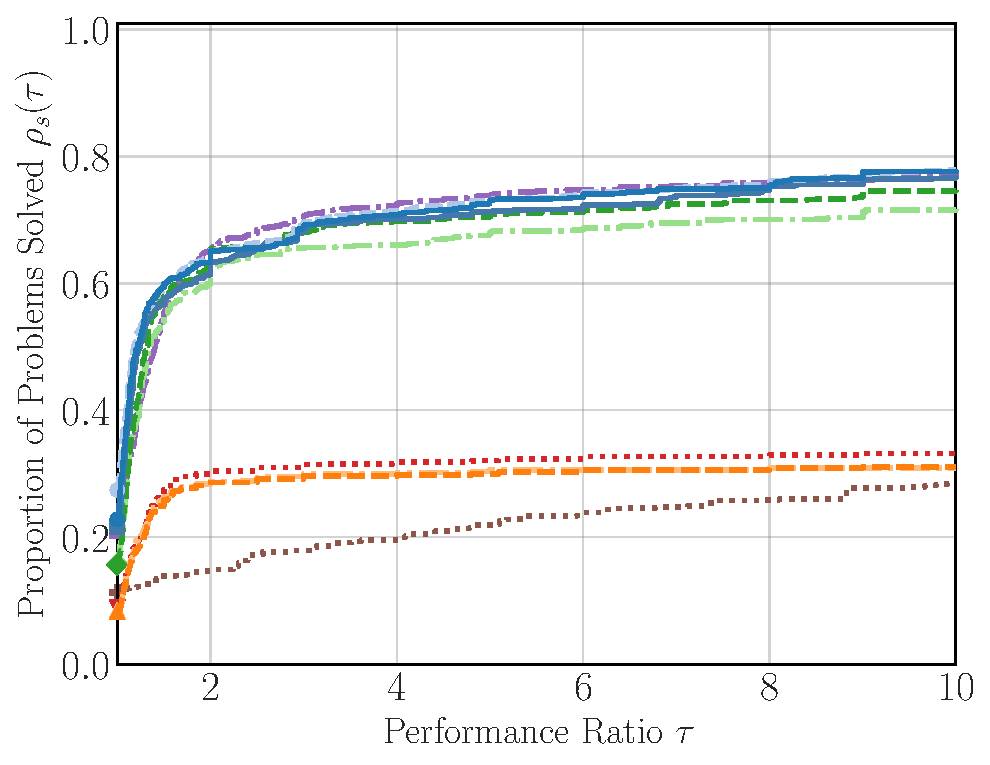
\includegraphics[width=\textwidth]{../imgs/compare/_pp_function_only_gtol1e-02.pdf}
    \end{subfigure}
    \begin{subfigure}[b]{0.98\textwidth}
        \centering
        
\includegraphics[width=\textwidth]{../imgs/compare/_legend_noise.pdf}
    \end{subfigure}
    \caption{Theory-aligned function-value-noise results at noise level $10^{-3}$, supplied error bound \(\feps = 10^{-2}\), and \(\gtol = 10^{-2}\).}
    \label{fig:results_function_noise}
\end{figure}
\end{MPCchange}

\begin{figure}[t]
    \centering
    \begin{subfigure}[b]{0.72\textwidth}
        \centering
        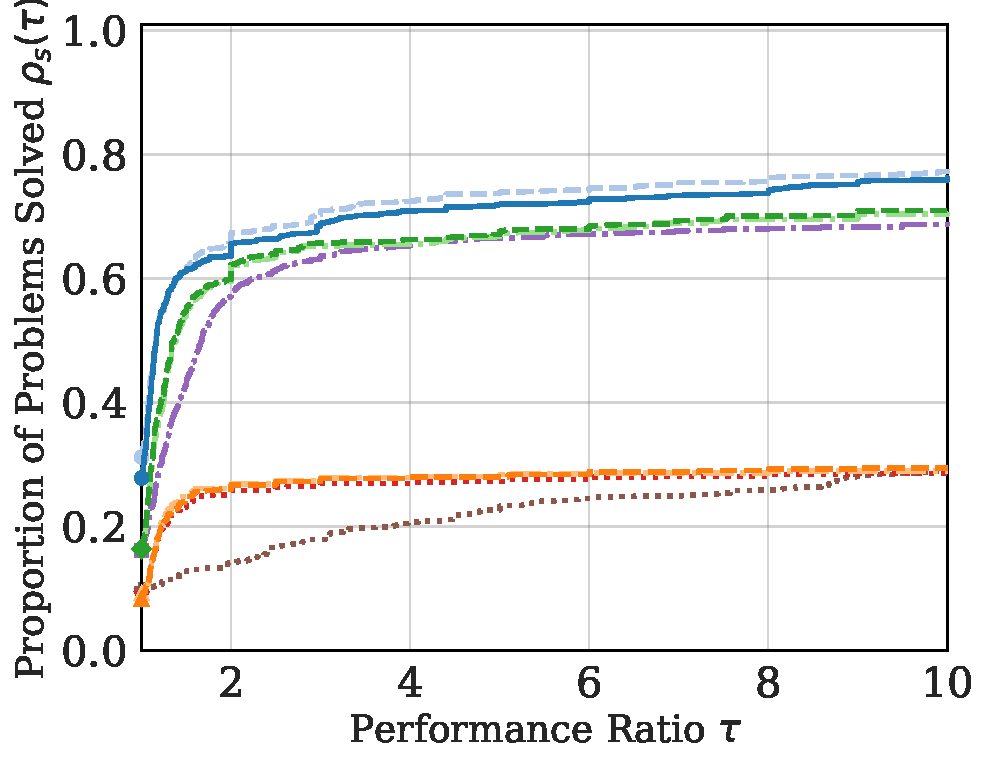
\includegraphics[width=\textwidth]{../imgs/compare/_pp_noise0.001_gtol1e-02.pdf}
    \end{subfigure}
    \begin{subfigure}[b]{0.98\textwidth}
        \centering
        
\includegraphics[width=\textwidth]{../imgs/compare/_legend_noise.pdf}
    \end{subfigure}
    \caption{Performance profile for \MPCchanged{the deliberately adverse joint function-and-gradient} noise setting \MPCchanged{(componentwise level \(10^{-3}\))} and $\gtol=10^{-2}$\MPCchanged{.
    This experiment lies outside the exact-gradient theory}.}
    \label{fig:results_noise}
\end{figure}

\begin{MPCchange}
\begin{figure}[t]
    \ifdefined\MPCRevision\captionsetup{font={color=red}}\fi
    \centering
    \begin{subfigure}[b]{0.32\textwidth}
        \centering
        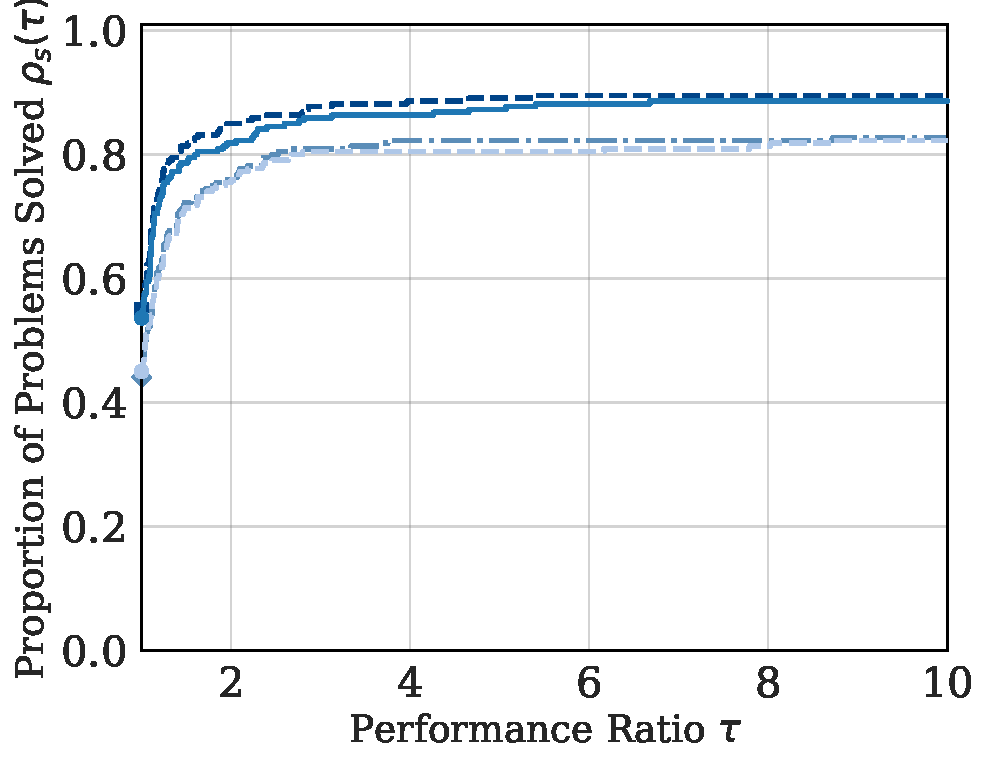
\includegraphics[width=\textwidth]{../imgs/compare/_pp_eps_under_gtol1e-02.pdf}
        \caption{\(\feps = 10^{-4}\).}
    \end{subfigure}
    \hfill
    \begin{subfigure}[b]{0.32\textwidth}
        \centering
        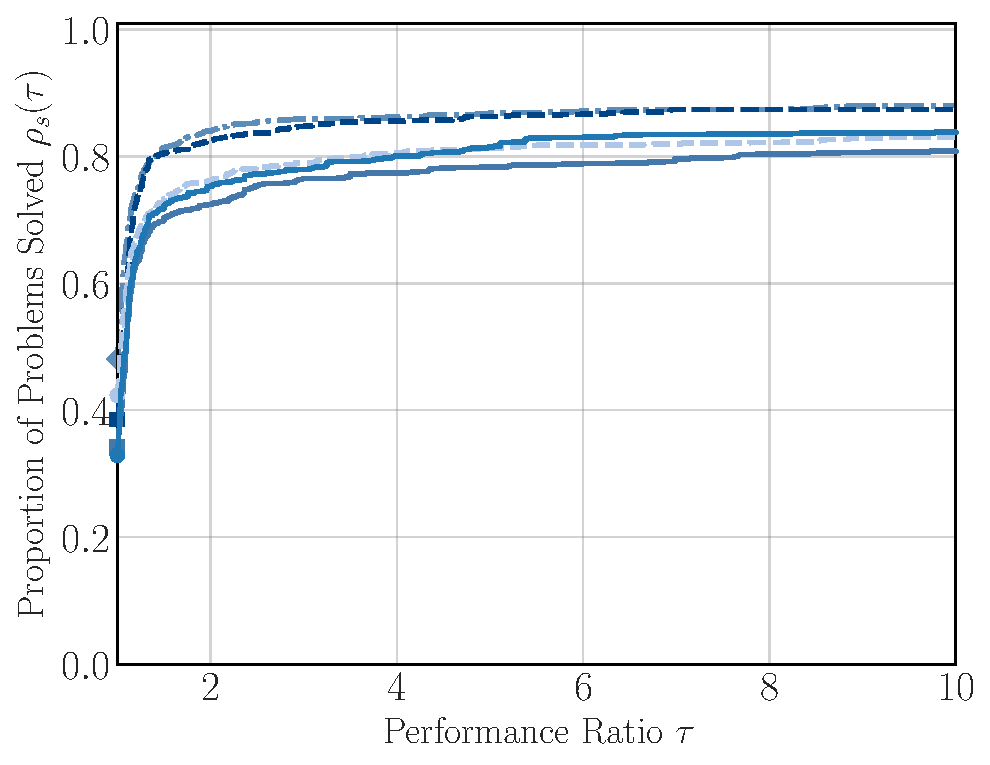
\includegraphics[width=\textwidth]{../imgs/compare/_pp_eps_nominal_gtol1e-02.pdf}
        \caption{\(\feps = 10^{-2}\).}
    \end{subfigure}
    \hfill
    \begin{subfigure}[b]{0.32\textwidth}
        \centering
        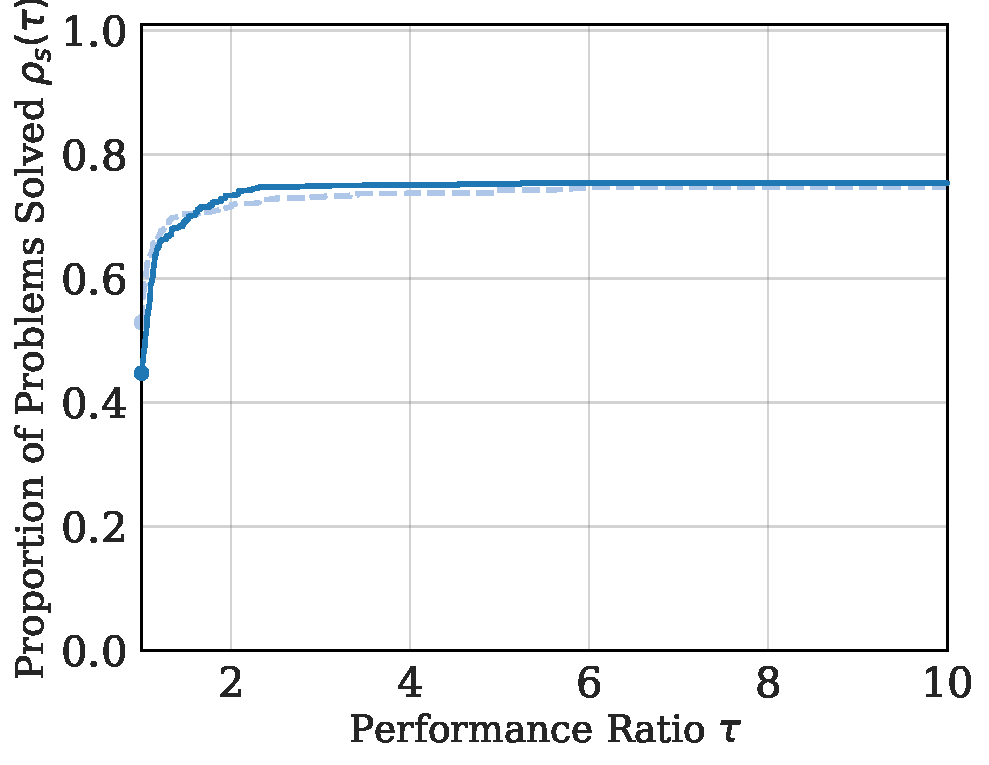
\includegraphics[width=\textwidth]{../imgs/compare/_pp_eps_over_gtol1e-02.pdf}
        \caption{\(\feps = 10^{-1}\).}
    \end{subfigure}
    \begin{subfigure}[b]{0.98\textwidth}
        \centering
        
\includegraphics[width=\textwidth]{../imgs/compare/_legend_sensitivity.pdf}
    \end{subfigure}
    \caption{Performance profiles for error-bound misspecification under function-value-only noise of level $10^{-3}$ and \(\gtol = 10^{-2}\).}
    \label{fig:results_error_bound_sensitivity}
\end{figure}
\end{MPCchange}

\subsubsection{Results at Different Precision Levels}\label{sssec:exact_results}

We next present performance profiles for each floating-point precision (64-, 32-, and 16-bit).
We evaluated each method at three gradient norm tolerance levels, i.e., $\gtol \in \{10^{-1}, 10^{-3}, 10^{-5}\}$.
These tolerance levels represent different optimization regimes, from moderate accuracy to high precision requirements.
\Cref{fig:results_all_precisions} shows the comprehensive performance profiles across all three precision levels.
\begin{MPCchange}
At the strictest tolerance \(\gtol = 10^{-5}\), \texttt{Ours} and \texttt{Ours-MS} solve $84.5\%$ and $85.5\%$ of the 64-bit problems, $52.3\%$ and $52.7\%$ of the 32-bit problems, and $28.9\%$ and $28.9\%$ of the 16-bit problems.
The decreasing rates quantify the expected loss of attainable accuracy as arithmetic precision is reduced, while both variants remain among the most robust methods in the profiles.
Their relative ranking depends on the tolerance and precision, so we avoid claiming uniform superiority and report both the fraction solved and the performance ratios in \cref{fig:results_all_precisions}.
\end{MPCchange}

\begin{figure}[t]
    \centering
    % 64-bit precision
    \begin{subfigure}[b]{\resultsAllPrecisionsSubfigWidth\textwidth}
        \centering
        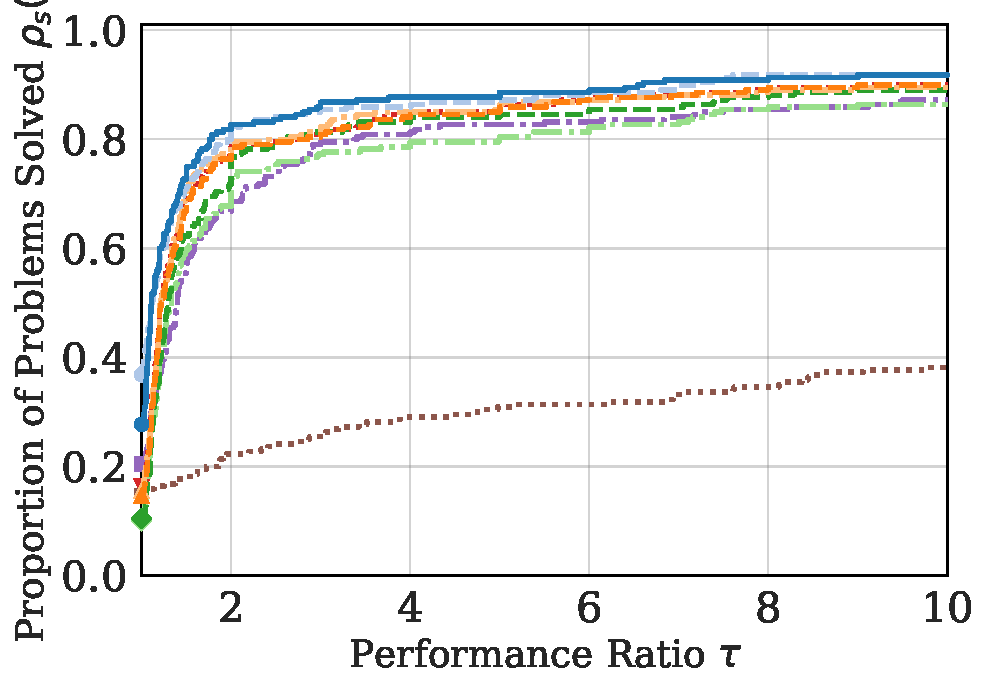
\includegraphics[width=\textwidth]{../imgs/compare/_pp_precision64_gtol1e-01.pdf}
        \caption{64-bit, $\gtol=10^{-1}$}
    \end{subfigure}
    \hfill
    \begin{subfigure}[b]{\resultsAllPrecisionsSubfigWidth\textwidth}
        \centering
        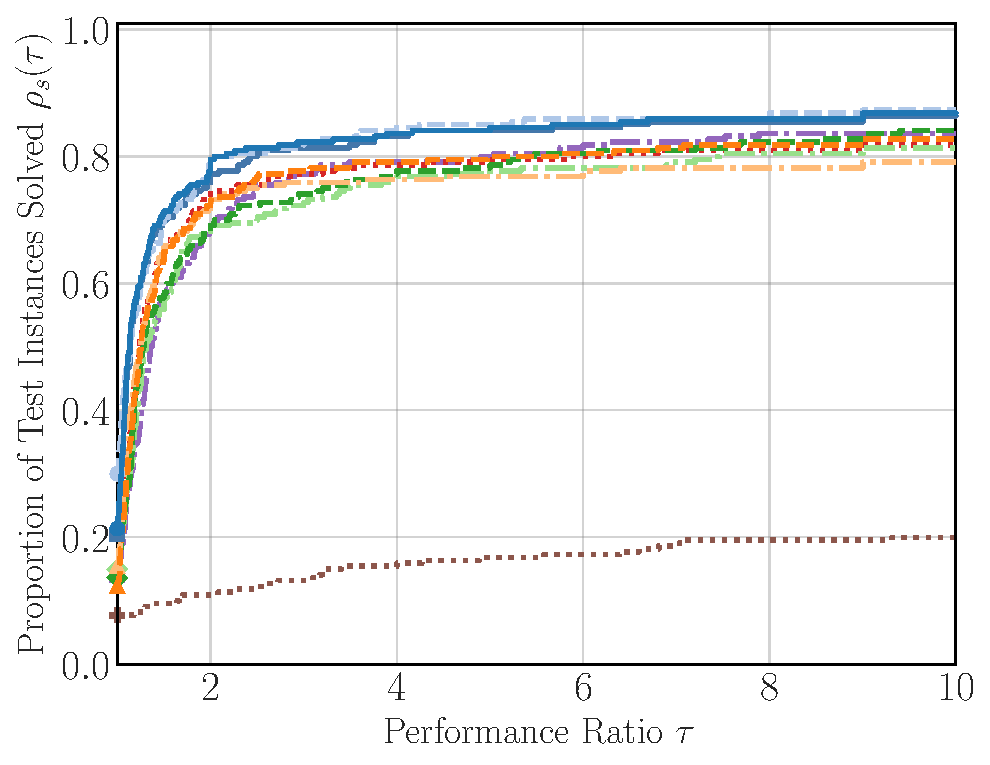
\includegraphics[width=\textwidth]{../imgs/compare/_pp_precision64_gtol1e-03.pdf}
        \caption{64-bit, $\gtol=10^{-3}$}
    \end{subfigure}
    \hfill
    \begin{subfigure}[b]{\resultsAllPrecisionsSubfigWidth\textwidth}
        \centering
        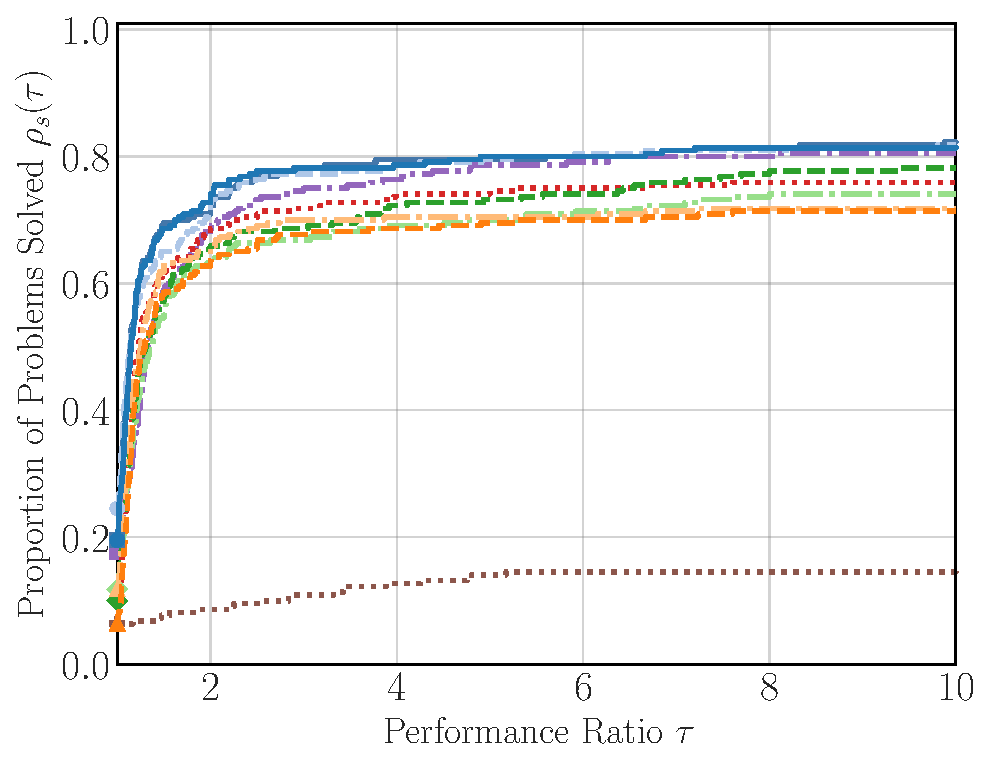
\includegraphics[width=\textwidth]{../imgs/compare/_pp_precision64_gtol1e-05.pdf}
        \caption{64-bit, $\gtol=10^{-5}$}
    \end{subfigure}

    \vspace{0.5em}

    % 32-bit precision
    \begin{subfigure}[b]{\resultsAllPrecisionsSubfigWidth\textwidth}
        \centering
        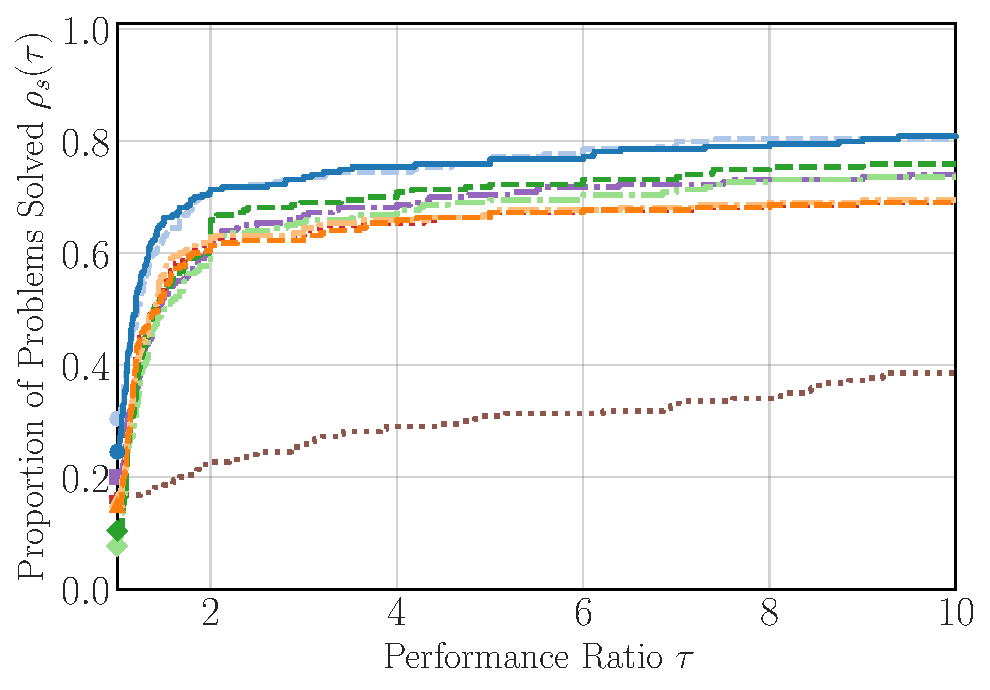
\includegraphics[width=\textwidth]{../imgs/compare/_pp_precision32_gtol1e-01.pdf}
        \caption{32-bit, $\gtol=10^{-1}$}
    \end{subfigure}
    \hfill
    \begin{subfigure}[b]{\resultsAllPrecisionsSubfigWidth\textwidth}
        \centering
        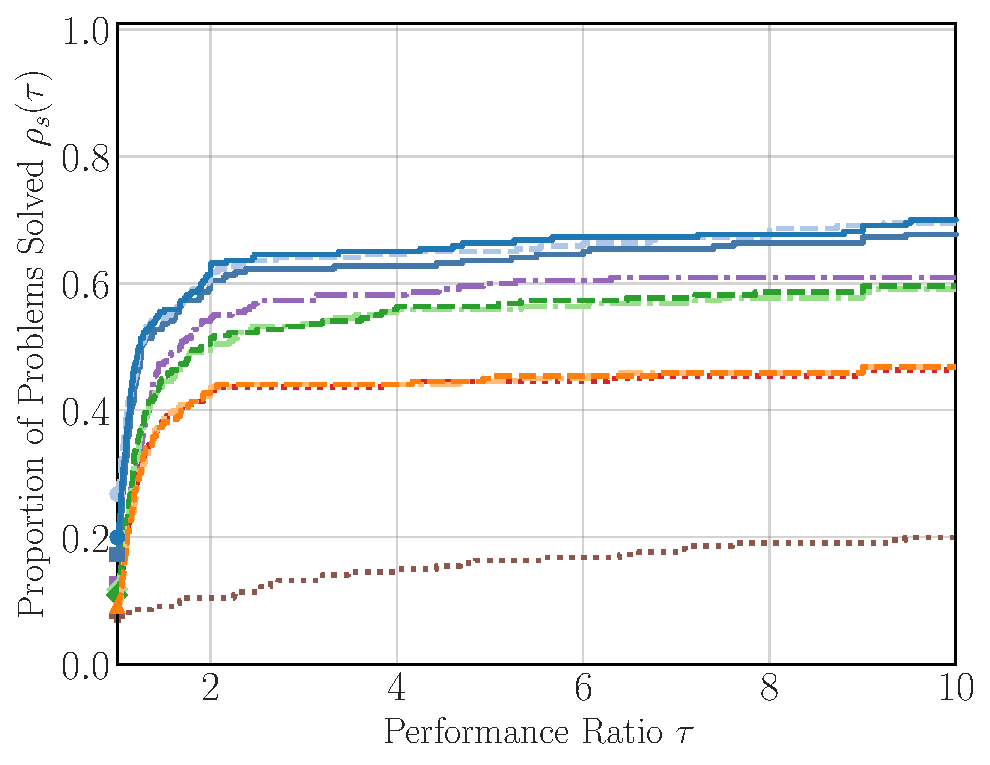
\includegraphics[width=\textwidth]{../imgs/compare/_pp_precision32_gtol1e-03.pdf}
        \caption{32-bit, $\gtol=10^{-3}$}
    \end{subfigure}
    \hfill
    \begin{subfigure}[b]{\resultsAllPrecisionsSubfigWidth\textwidth}
        \centering
        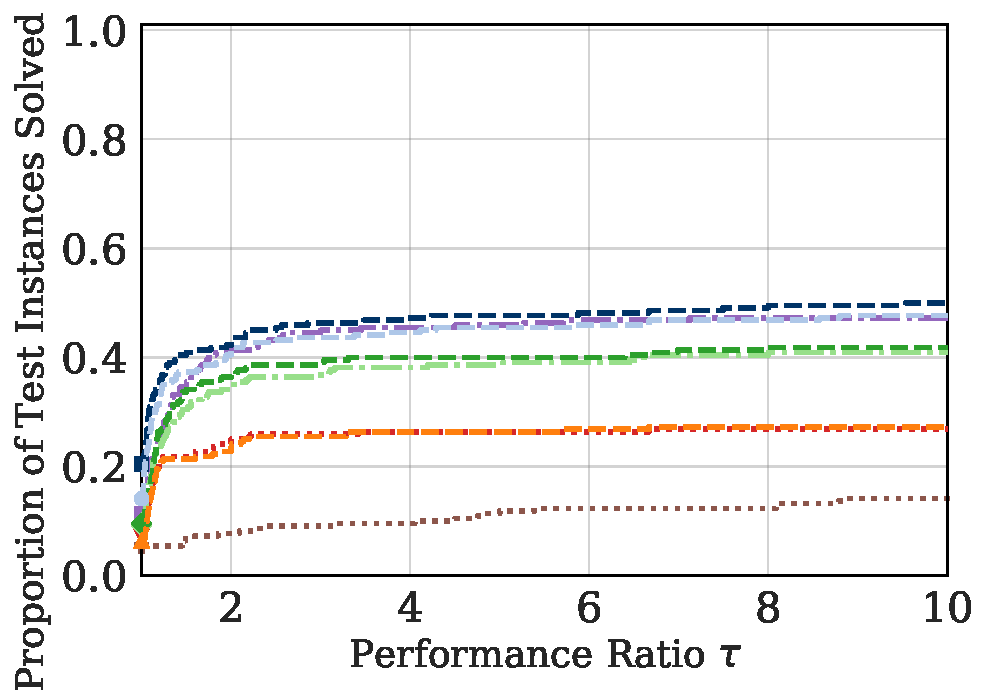
\includegraphics[width=\textwidth]{../imgs/compare/_pp_precision32_gtol1e-05.pdf}
        \caption{32-bit, $\gtol=10^{-5}$}
    \end{subfigure}

    \vspace{0.5em}

    % 16-bit precision
    \begin{subfigure}[b]{\resultsAllPrecisionsSubfigWidth\textwidth}
        \centering
        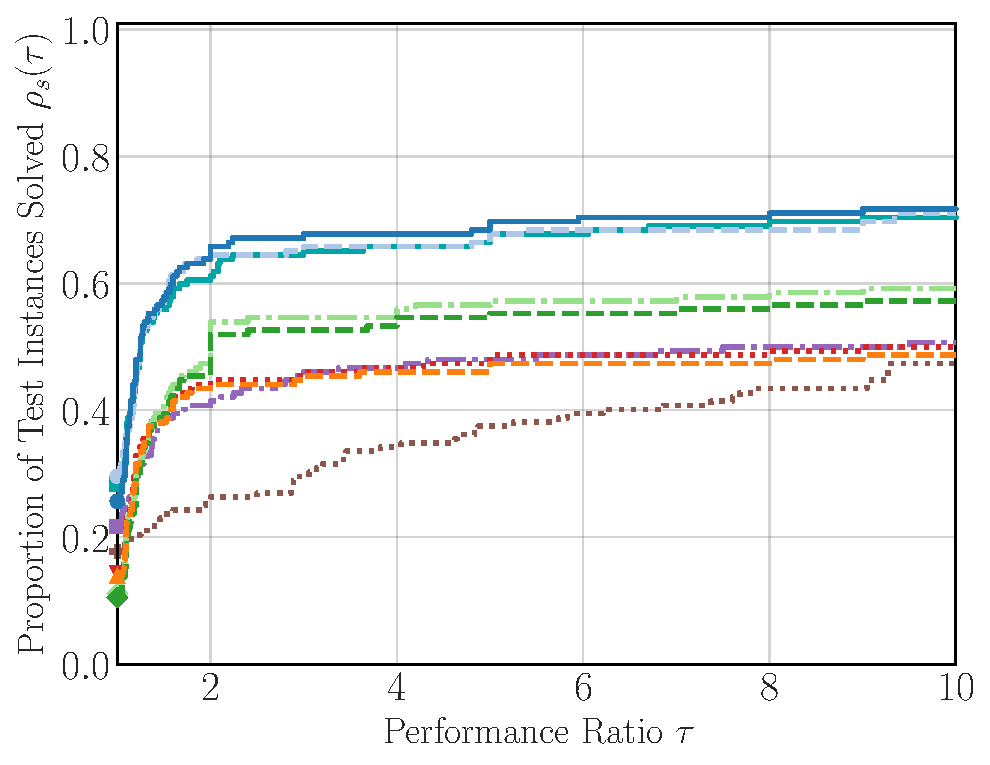
\includegraphics[width=\textwidth]{../imgs/compare/_pp_precision16_gtol1e-01.pdf}
        \caption{16-bit, $\gtol=10^{-1}$}
    \end{subfigure}
    \hfill
    \begin{subfigure}[b]{\resultsAllPrecisionsSubfigWidth\textwidth}
        \centering
        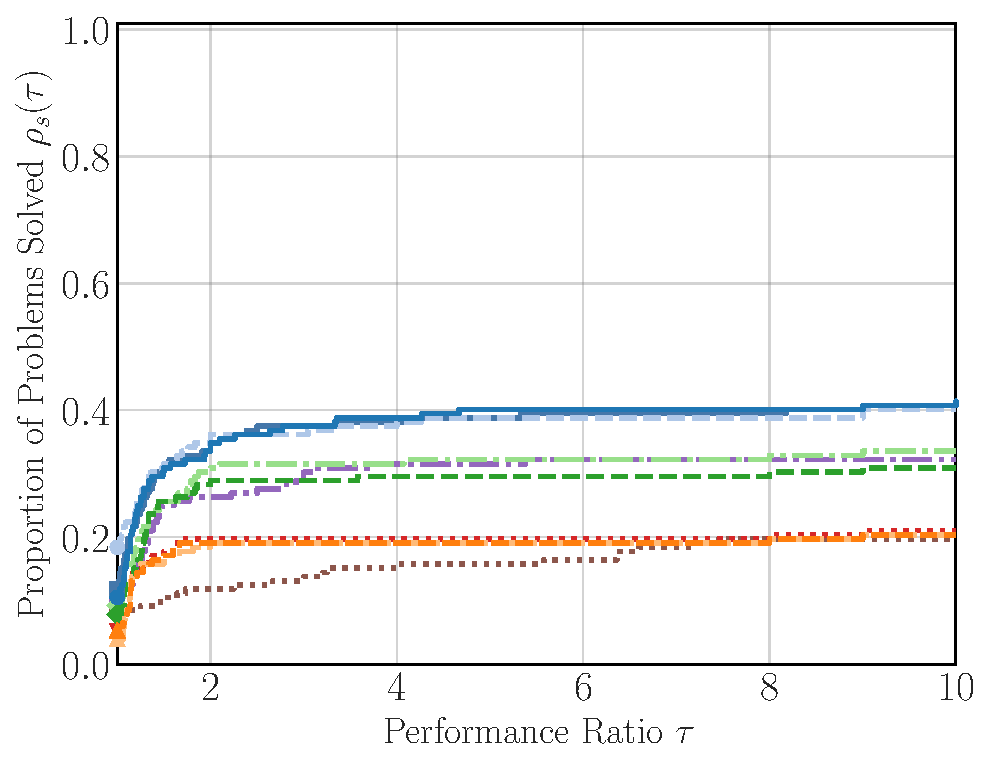
\includegraphics[width=\textwidth]{../imgs/compare/_pp_precision16_gtol1e-03.pdf}
        \caption{16-bit, $\gtol=10^{-3}$}
    \end{subfigure}
    \hfill
    \begin{subfigure}[b]{\resultsAllPrecisionsSubfigWidth\textwidth}
        \centering
        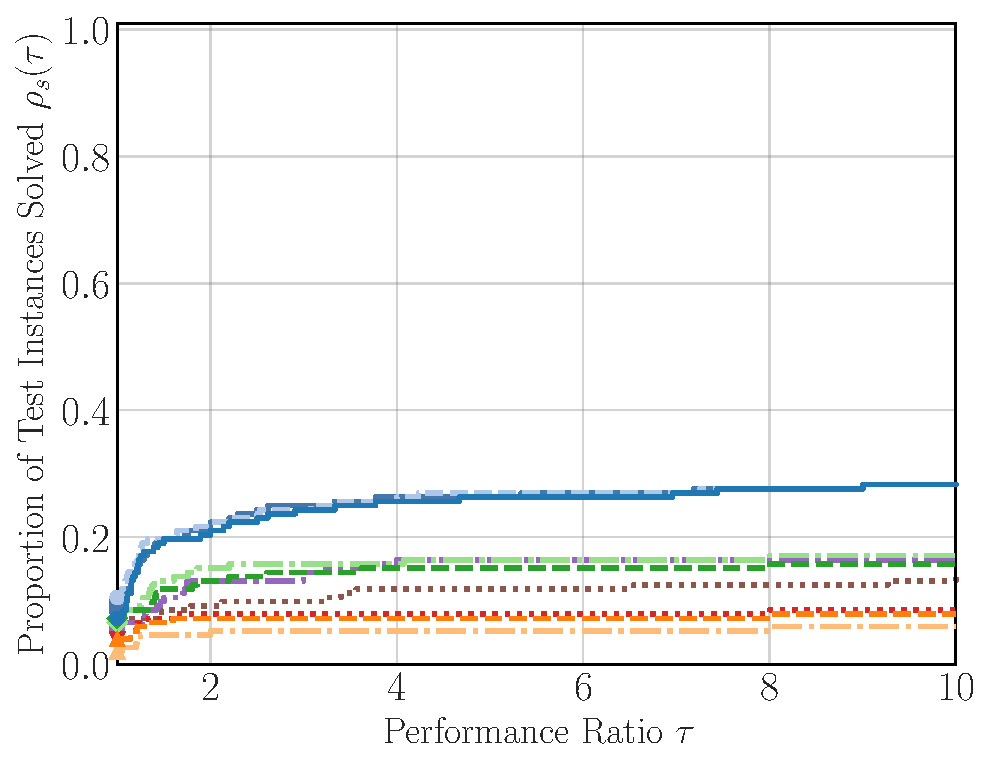
\includegraphics[width=\textwidth]{../imgs/compare/_pp_precision16_gtol1e-05.pdf}
        \caption{16-bit, $\gtol=10^{-5}$}
    \end{subfigure}

    \vspace{0.5em}

    % Legend
    \begin{subfigure}[b]{0.98\textwidth}
        \centering
        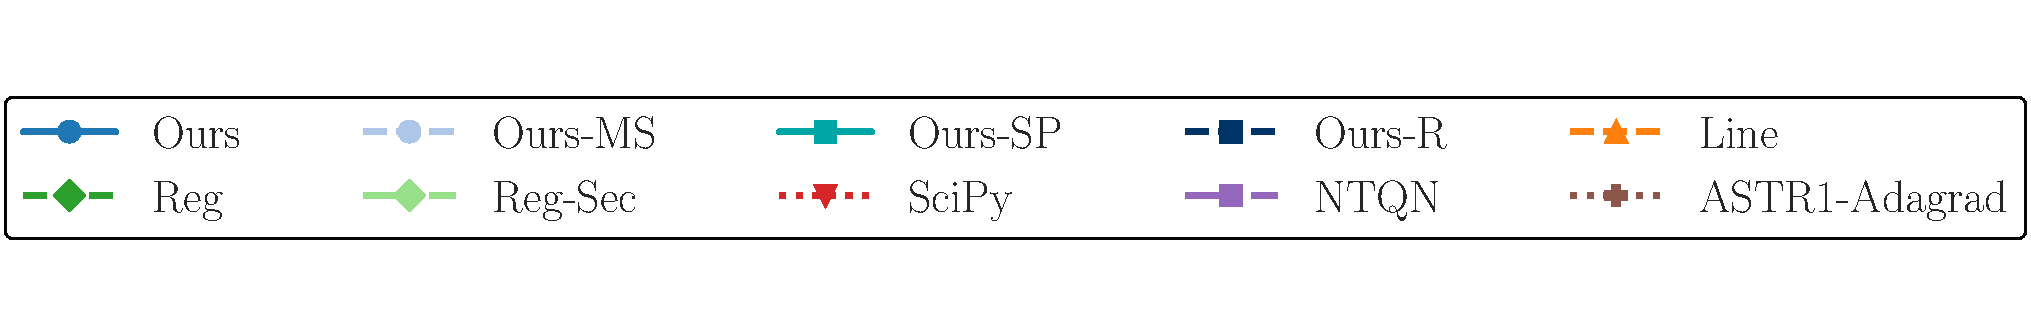
\includegraphics[width=\textwidth]{../imgs/compare/_legend_precision.pdf}
    \end{subfigure}
    \caption{\MPCchanged{Performance profiles across floating-point precisions (64-, 32-, and 16-bit) and tolerance levels.}}
    \label{fig:results_all_precisions}
\end{figure}

\subsection{Computational Time per Iteration}\label{sec:comp_time}

\begin{figure}[t]
    \centering
    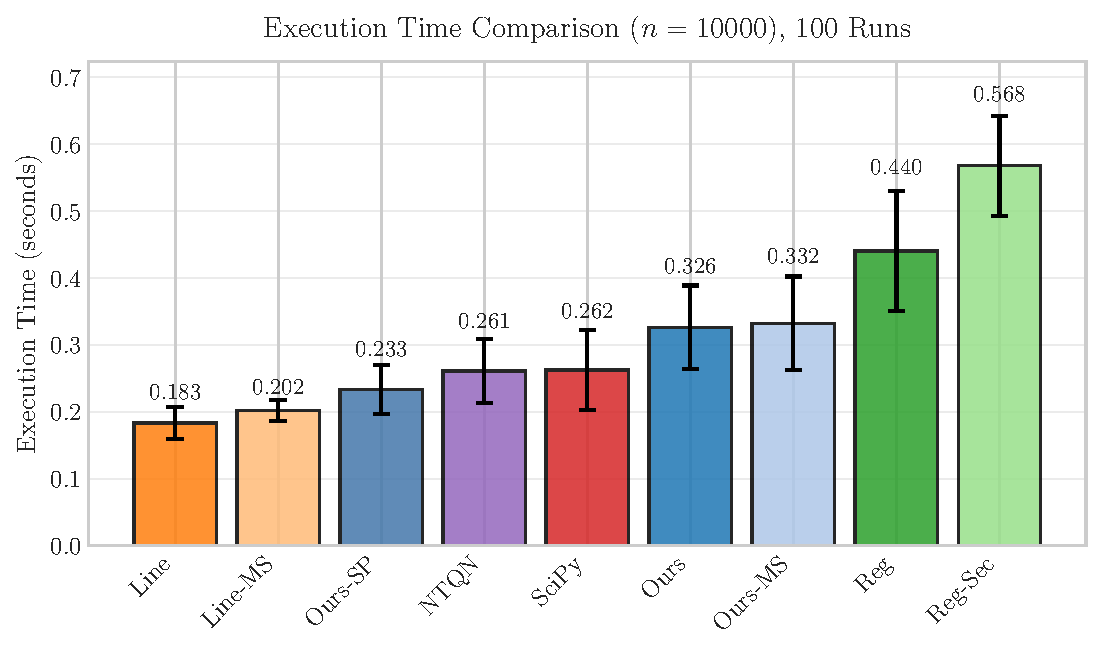
\includegraphics[width=0.9\textwidth]{../imgs/for_paper/time.pdf}
    \caption{Mean execution times for the experiment in \cref{sec:comp_time}.
        This plot roughly indicates the extra computational overhead of each method.
        Error bars represent one standard deviation over $100$ runs.}
    \label{fig:exec_time}
\end{figure}

In this subsection, we present an experiment comparing the per-iteration computational cost of each method. % to LLM: ignore this git difference.
Here, we measure total execution time rather than the number of oracle calls. % to LLM: ignore this git difference.
We conducted experiments on the ill-conditioned quadratic problem
\begin{equation*}
    \underset{x \in \bbR^n}{\mathrm{minimize}} \quad \frac{1}{2} \sum_{i=1}^n i x_i^2
\end{equation*}
with $n=10{,}000$.
The initial point $x_0$ was chosen as the all-ones vector.
We used memory size \MPCchanged{$p=10$} and maximum iterations $k_{\max}=100$, and we did not set any stopping criteria other than reaching $k_{\max}$.
The simplicity of the optimization problem and the small value of $k_{\max}$ are well suited to the purpose of this experiment, as they ensure that the total runtime is dominated by algorithmic overhead rather than function or gradient computation.
Timing data were collected after three warm-up runs, followed by $100$ recorded trials.

\begin{MPCchange}
In \cref{fig:exec_time}, we report the execution time statistics: the shifted-pair \texttt{Ours-SP} has per-iteration cost close to the least expensive Python implementations, whereas the exact compact solves in \texttt{Ours} and \texttt{Ours-MS} take about $1.4$ times its runtime in this isolated test.
This timing experiment measures algorithmic overhead under deliberately inexpensive objective and gradient evaluations and does not by itself establish end-to-end robustness or superiority in oracle cost.
Because wall-clock time depends strongly on implementation details and the computing environment, we restrict its interpretation to this isolated experiment and do not draw broader conclusions from the timing results.
For a fairer comparison of algorithmic efficiency, we place greater emphasis on oracle-call counts and success profiles.

In \cref{tab:time_results}, we report the total number of oracle calls (calls of $\overline{f}$ and $g$) and final objective values $\overline{f}(x_{k_{\max}})$.
\end{MPCchange}
\MPCchanged{To further check that the timing comparison is not driven only by a small fixed overhead or by fluctuations in very short runs, we report the 64-bit performance profile at $\gtol = 10^{-3}$ separately for three runtime ranges.}
\MPCchanged{In \cref{fig:time_ranges}, problem instances are grouped according to the best runtime attained by any method: less than $1$~s, between $1$ and $10$~s, and at least $10$~s.}
\MPCchanged{The three panels show the same overall tendency as the existing experiments and indicate that the reported per-iteration timing is not merely an artifact of short-run overhead.}
\MPCchanged{The other parameter settings exhibit qualitatively similar behavior.}

\begin{MPCchange}
\begin{figure}[t]
    \ifdefined\MPCRevision\captionsetup{font={color=red}}\fi
    \centering
    \begin{subfigure}[b]{0.32\textwidth}
        \centering
        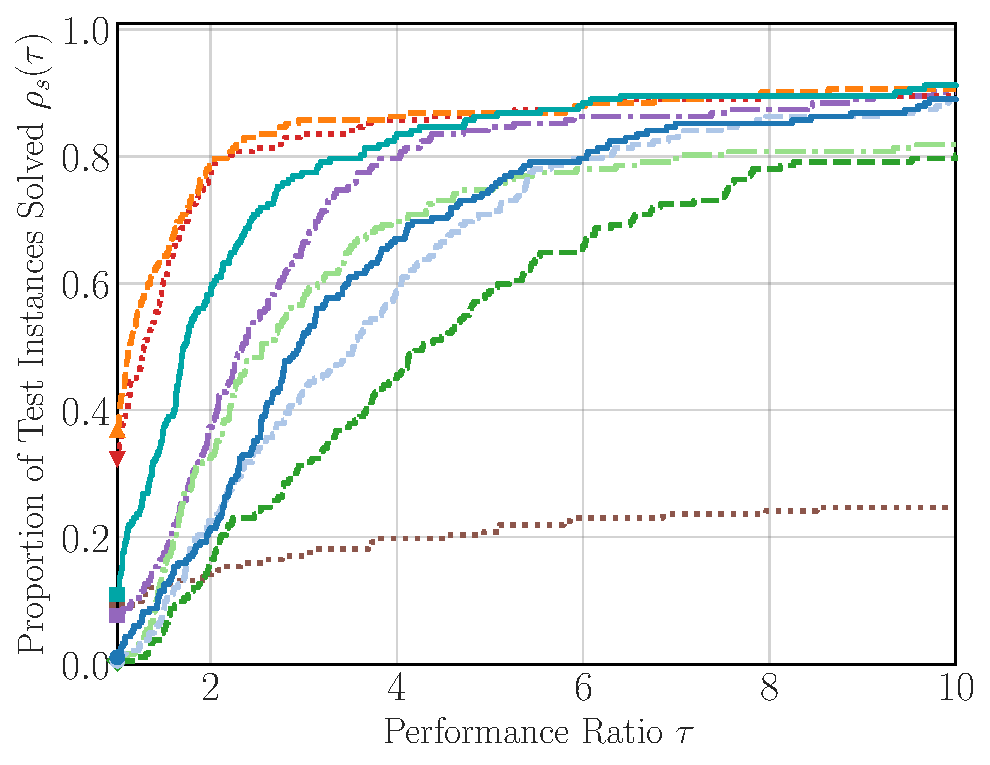
\includegraphics[width=\textwidth]{../imgs/compare/_pp_precision64_gtol1e-03_time_lt1s.pdf}
        \caption{Less than $1$~s.}
    \end{subfigure}
    \hfill
    \begin{subfigure}[b]{0.32\textwidth}
        \centering
        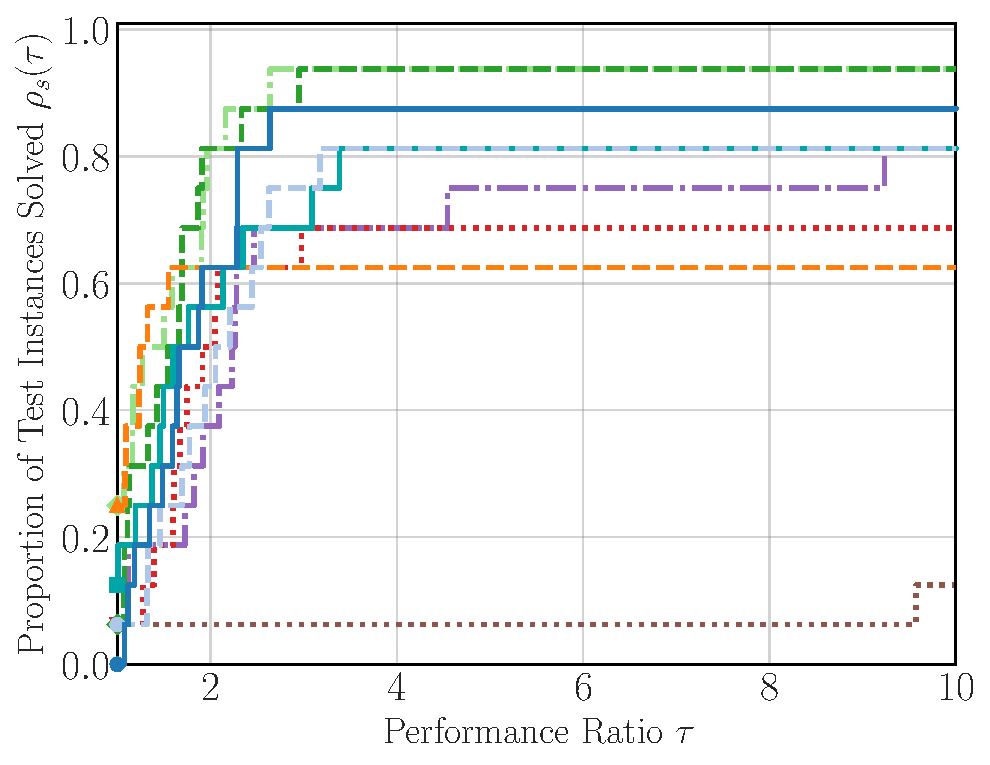
\includegraphics[width=\textwidth]{../imgs/compare/_pp_precision64_gtol1e-03_time_1-10s.pdf}
        \caption{Between $1$ and $10$~s.}
    \end{subfigure}
    \hfill
    \begin{subfigure}[b]{0.32\textwidth}
        \centering
        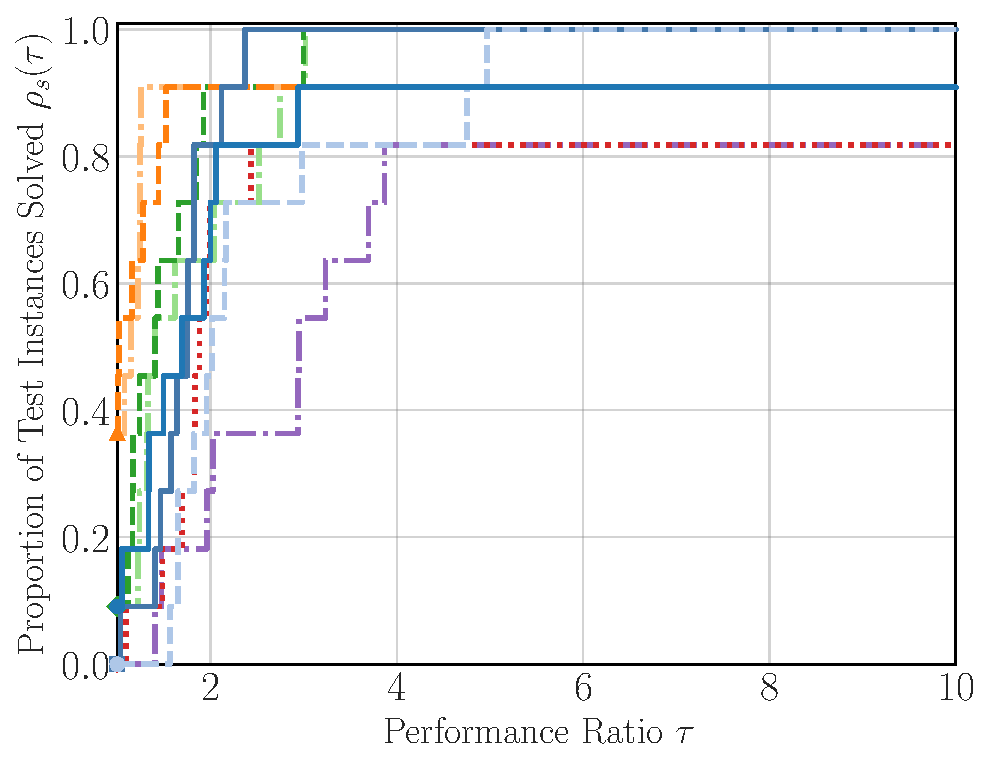
\includegraphics[width=\textwidth]{../imgs/compare/_pp_precision64_gtol1e-03_time_ge10s.pdf}
        \caption{At least $10$~s.}
    \end{subfigure}
    \begin{subfigure}[b]{0.98\textwidth}
        \centering
        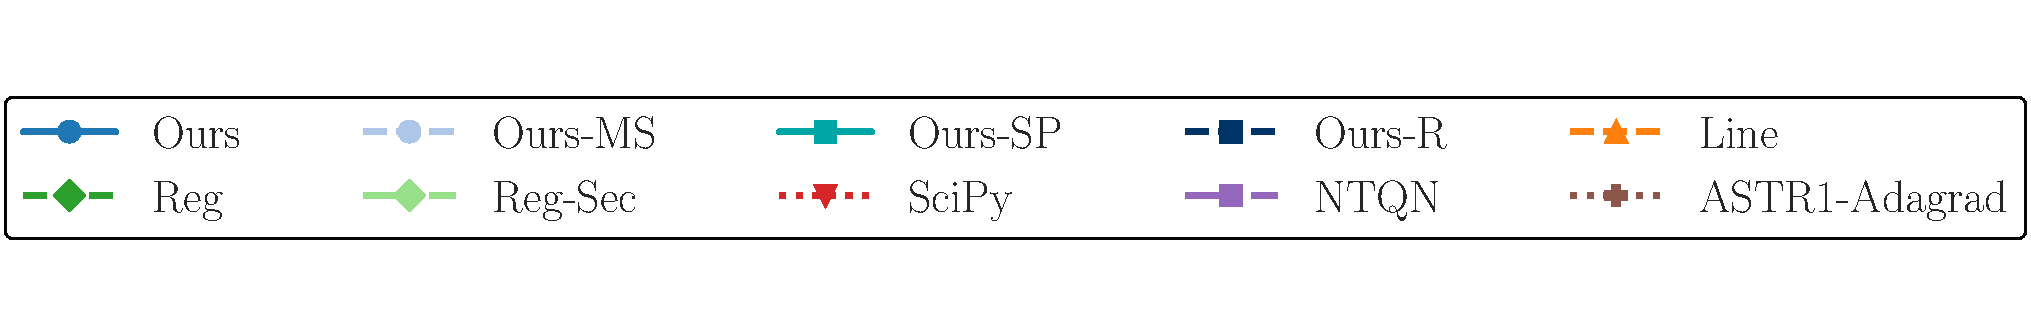
\includegraphics[width=\textwidth]{../imgs/compare/_legend_precision.pdf}
    \end{subfigure}
    \caption{Performance profiles for the 64-bit setting at $\gtol = 10^{-3}$, grouped by the best runtime attained by any method on each problem instance.}
    \label{fig:time_ranges}
\end{figure}
\end{MPCchange}

\MPCchanged{The purpose of this table is to check whether the methods achieved similar convergence behavior within the limited number of iterations.}
\MPCchanged{Comparable values would indicate that differences in convergence behavior do not dominate the execution-time comparison.}

\begin{table}[t]
    \centering
    \small
    \setlength{\tabcolsep}{3.5pt}
    \caption{The number of oracle calls and final observed objective values for the experiment in \cref{sec:comp_time}.}
    \label{tab:time_results}
    \begin{tabular}{lrrrrrrrrr}
    \toprule
                                & \texttt{Line} & \texttt{Line-MS} & \texttt{Ours-SP} & \texttt{NTQN} & \texttt{Reg} & \texttt{SciPy} & \texttt{Reg-Sec} & \texttt{Ours} & \texttt{Ours-MS} \\
    \midrule
            \# Calls & 212 & 212 & 202 & 219 & 206 & 212 & 206 & 202 & 202 \\
    $\overline{f}(x_{k_{\max}})$ & 1.24 & 1.24 & 1.34 & 1.43 & 1.47 & 1.24 & 1.48 & 1.34 & 1.34 \\
    \bottomrule
    \end{tabular}
\end{table}


\section{Conclusion}\label{sec:conclusion}

\MPCchanged{We proposed a hybrid regularized quasi-Newton method for smooth nonconvex optimization with bounded errors in objective-function values.
The method retains the order-optimal \(\order{1/\varepsilon^2}\) first-order iteration complexity of the $L$-smooth nonconvex setting while selectively using noisy function values.}
\MPCchanged{On the tested CUTEst problems, the proposed variants attained the common gradient tolerances across the reported function-noise, joint-noise, and reduced-precision settings.}
\MPCchanged{These results provide empirical evidence for the method under the stated benchmark protocol.}

Future work includes the investigation of local convergence properties, the extension to constrained optimization, and the applications to practical problems in machine learning and scientific computing. Additionally, exploring adaptive strategies for selecting algorithmic parameters based on problem characteristics could further enhance the method's performance.
An explicit analysis of the effect of inexact gradient evaluations would also provide valuable insight into the method's robustness and guide further enhancements.

\ifSubfilesClassLoaded{
    \bibliographystyle{spbasic}
    \bibliography{../L-BFGS.bib}
}{}

\end{document}
